\chapter{System overview}\label{cha:overview}

In this chapter a system description is given. This is made for the reader to get a better understanding of the setup which was available at Aalborg University. This description includes the following points and will be described in the same order, then a summary of the system overview is provided.

\begin{itemize}
  \item The da Vinci robot,
  \item The EndoWrist,
  \item The mechanical test setup,  
  \item The motors,
  \item The embedded system,
  \item The Geomagic Touch
\end{itemize}
\todo{update itemizer later so it fits!}

\section{Da vinci robot}\label{sec:da_vin_rob}

The da Vinci robot is a minimal invasive surgery (MSI) robot used in surgeries such as cardiac, coloretal and gynecologic surgeries\cite{daVinciSurgery}. The version available at Aalborg University is a member of the first generation of da Vinci robots, see \figref{fig:fulldavinci}.

\begin{figure}[H]
	\centering
	\begin{subfigure}{.45\textwidth}
		\centering
		\includegraphics[width=\linewidth]{DavinciRobot.jpg}
		\caption{The da Vinci robot or slave manipulator.}
		\label{fig:davincirobot}
	\end{subfigure}
	\begin{subfigure}{.45\textwidth}
		\centering
		\vspace{12pt}
		\includegraphics[width=\linewidth]{masterconsole.jpg}
		\caption{The master console for controlling the slave manipulator.}
		\label{fig:mastermani}
	\end{subfigure}
\caption{Full view of the da Vinci surgery system which include the slave manipulator and the master console}
\label{fig:fulldavinci}
\end{figure}

It consists of two main parts, a master console, see \figref{fig:mastermani}, and a slave manipulator, see \figref{fig:davincirobot}.

\begin{itemize}
\item The surgeon uses the master console to control the slave manipulator. It consists of two eye pieces, which display a high resolution 3D view of the surgery for the surgeon. 
\item The slave manipulator is the robot which is controlled from the master console by the surgeon. It consists of four arms that with 6-7 actuated \gls{DOF} each, depending on the tool attached.
\end{itemize}

\textcolor{red}{The master console and three of the slave manipulator arms are disabled from the system. The console is disabled from the system, since force feedback is not an option on this device. The three arms are disabled since the control on these will be identical. The master console will not be further analyzed. To control the last arm on the slave manipulator, the Geomagic Touch, see \secref{sec:geo_magic}, has been implemented as replacement for the original master consol.}



%a replacement master controller called a Geo magic touch is implemented, see \secref{sec:geo_magic}.


\subsection*{Slave manipulator arm}
The slave manipulator arm consists of three parts, arm, hand and tool, see \figref{fig:davinciarmrobot}.

\begin{figure}[H]
	\centering
		\centering
		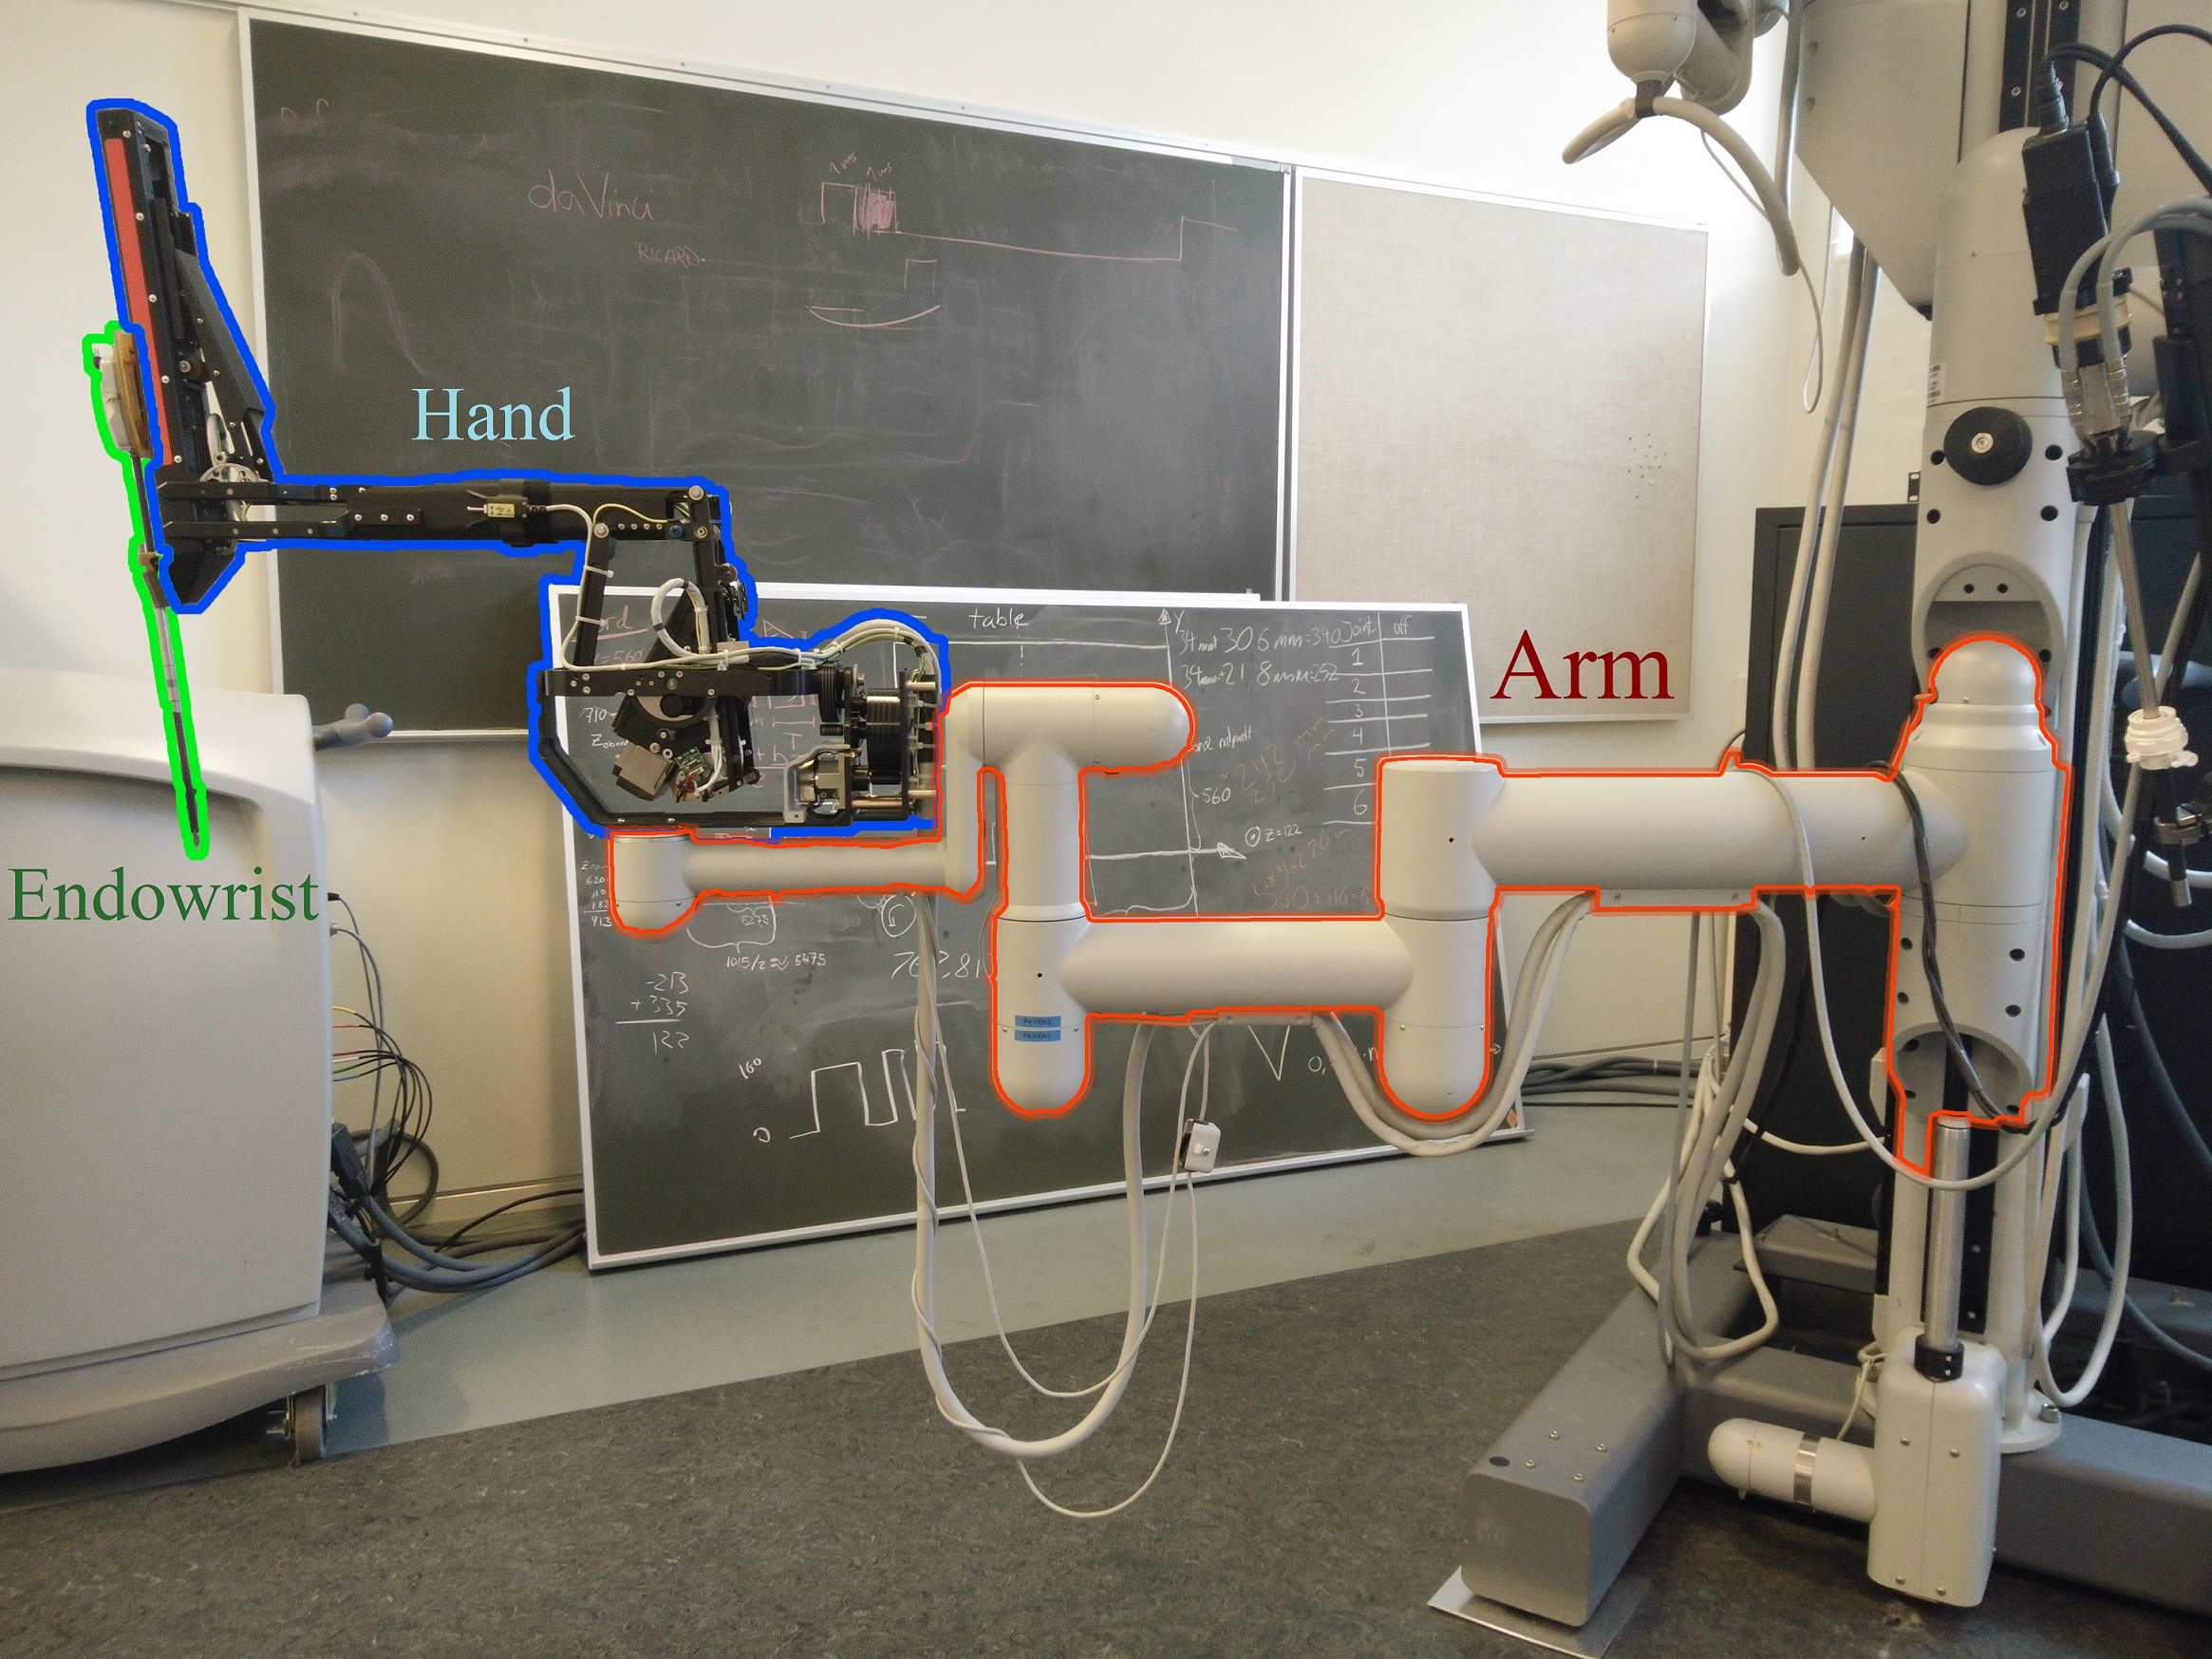
\includegraphics[width=0.85\linewidth]{davincirobotarm_label.jpg}
		\caption{One extended arm of the da Vinci robot. The tool (EndoWrist), hand and arm are marked.}
		\label{fig:davinciarmrobot}
\end{figure}


\begin{enumerate}
\item Arm:

The arm of the da Vinci is the part being the furthest away from the patient. 
During surgery, it is locked to a specific position. Between surgeries, its 6 \gls{DOF}s can be adjusted.
\item Hand

The hand is at the end of the arm and has three \gls{DOF}, two rotational and one translational, which can be actuated during surgery. 
\item End-effector tool (EndoWrist)

The end-effector tool is connected to the hand, it is only capable of doing rotational movement on its own. Together the tool and the hand have 6 - 7 movable \gls{DOF} that can be actuated. The tool is the instrument which interacts with the patient during surgery. There are several different tools available, each with their own functionality. 
\end{enumerate}

\textcolor{green}{The present project concentrates on implementing haptic feedback control for the end-effector called EndoWrist. Controlling the robot arm is not a subject of this project. The end-effector was separated from the da Vinci system. 
	
The da Vinci's master console controller lacks actuation. In order to be able to provide haptic feedback, a Geomagic Touch, see \secref{sec:geo_magic}, has been implemented as a replacement. The original master console will not be further analyzed. 	
}

\section{Endowrist}\label{sec:Endowrist}

An Endowrist, see \figref{fig:Endo_full} is a surgical tool which can be manipulated as a human wrist. It is used in surgical procedures such as Laparoscopic surgeries, better known as minimally invasive surgery (MIS), where small incisions in the human body is made under the surgery. Because the incision cuts are small, blood lose under the surgery and the risk of infection is reduced. This has a positive effect on the recovery time for the patient.


\begin{figure}[H]
	\centering
	\begin{subfigure}{.32\textwidth}
		\centering
		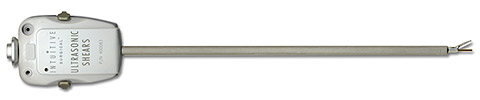
\includegraphics[width=\linewidth]{Endowrist1.jpg}
		\caption{Full view of a Endowrist\vspace{8.5mm}   }
		\label{fig:Endo_full}
	\end{subfigure}
	\begin{subfigure}{.32\textwidth}
		\centering
		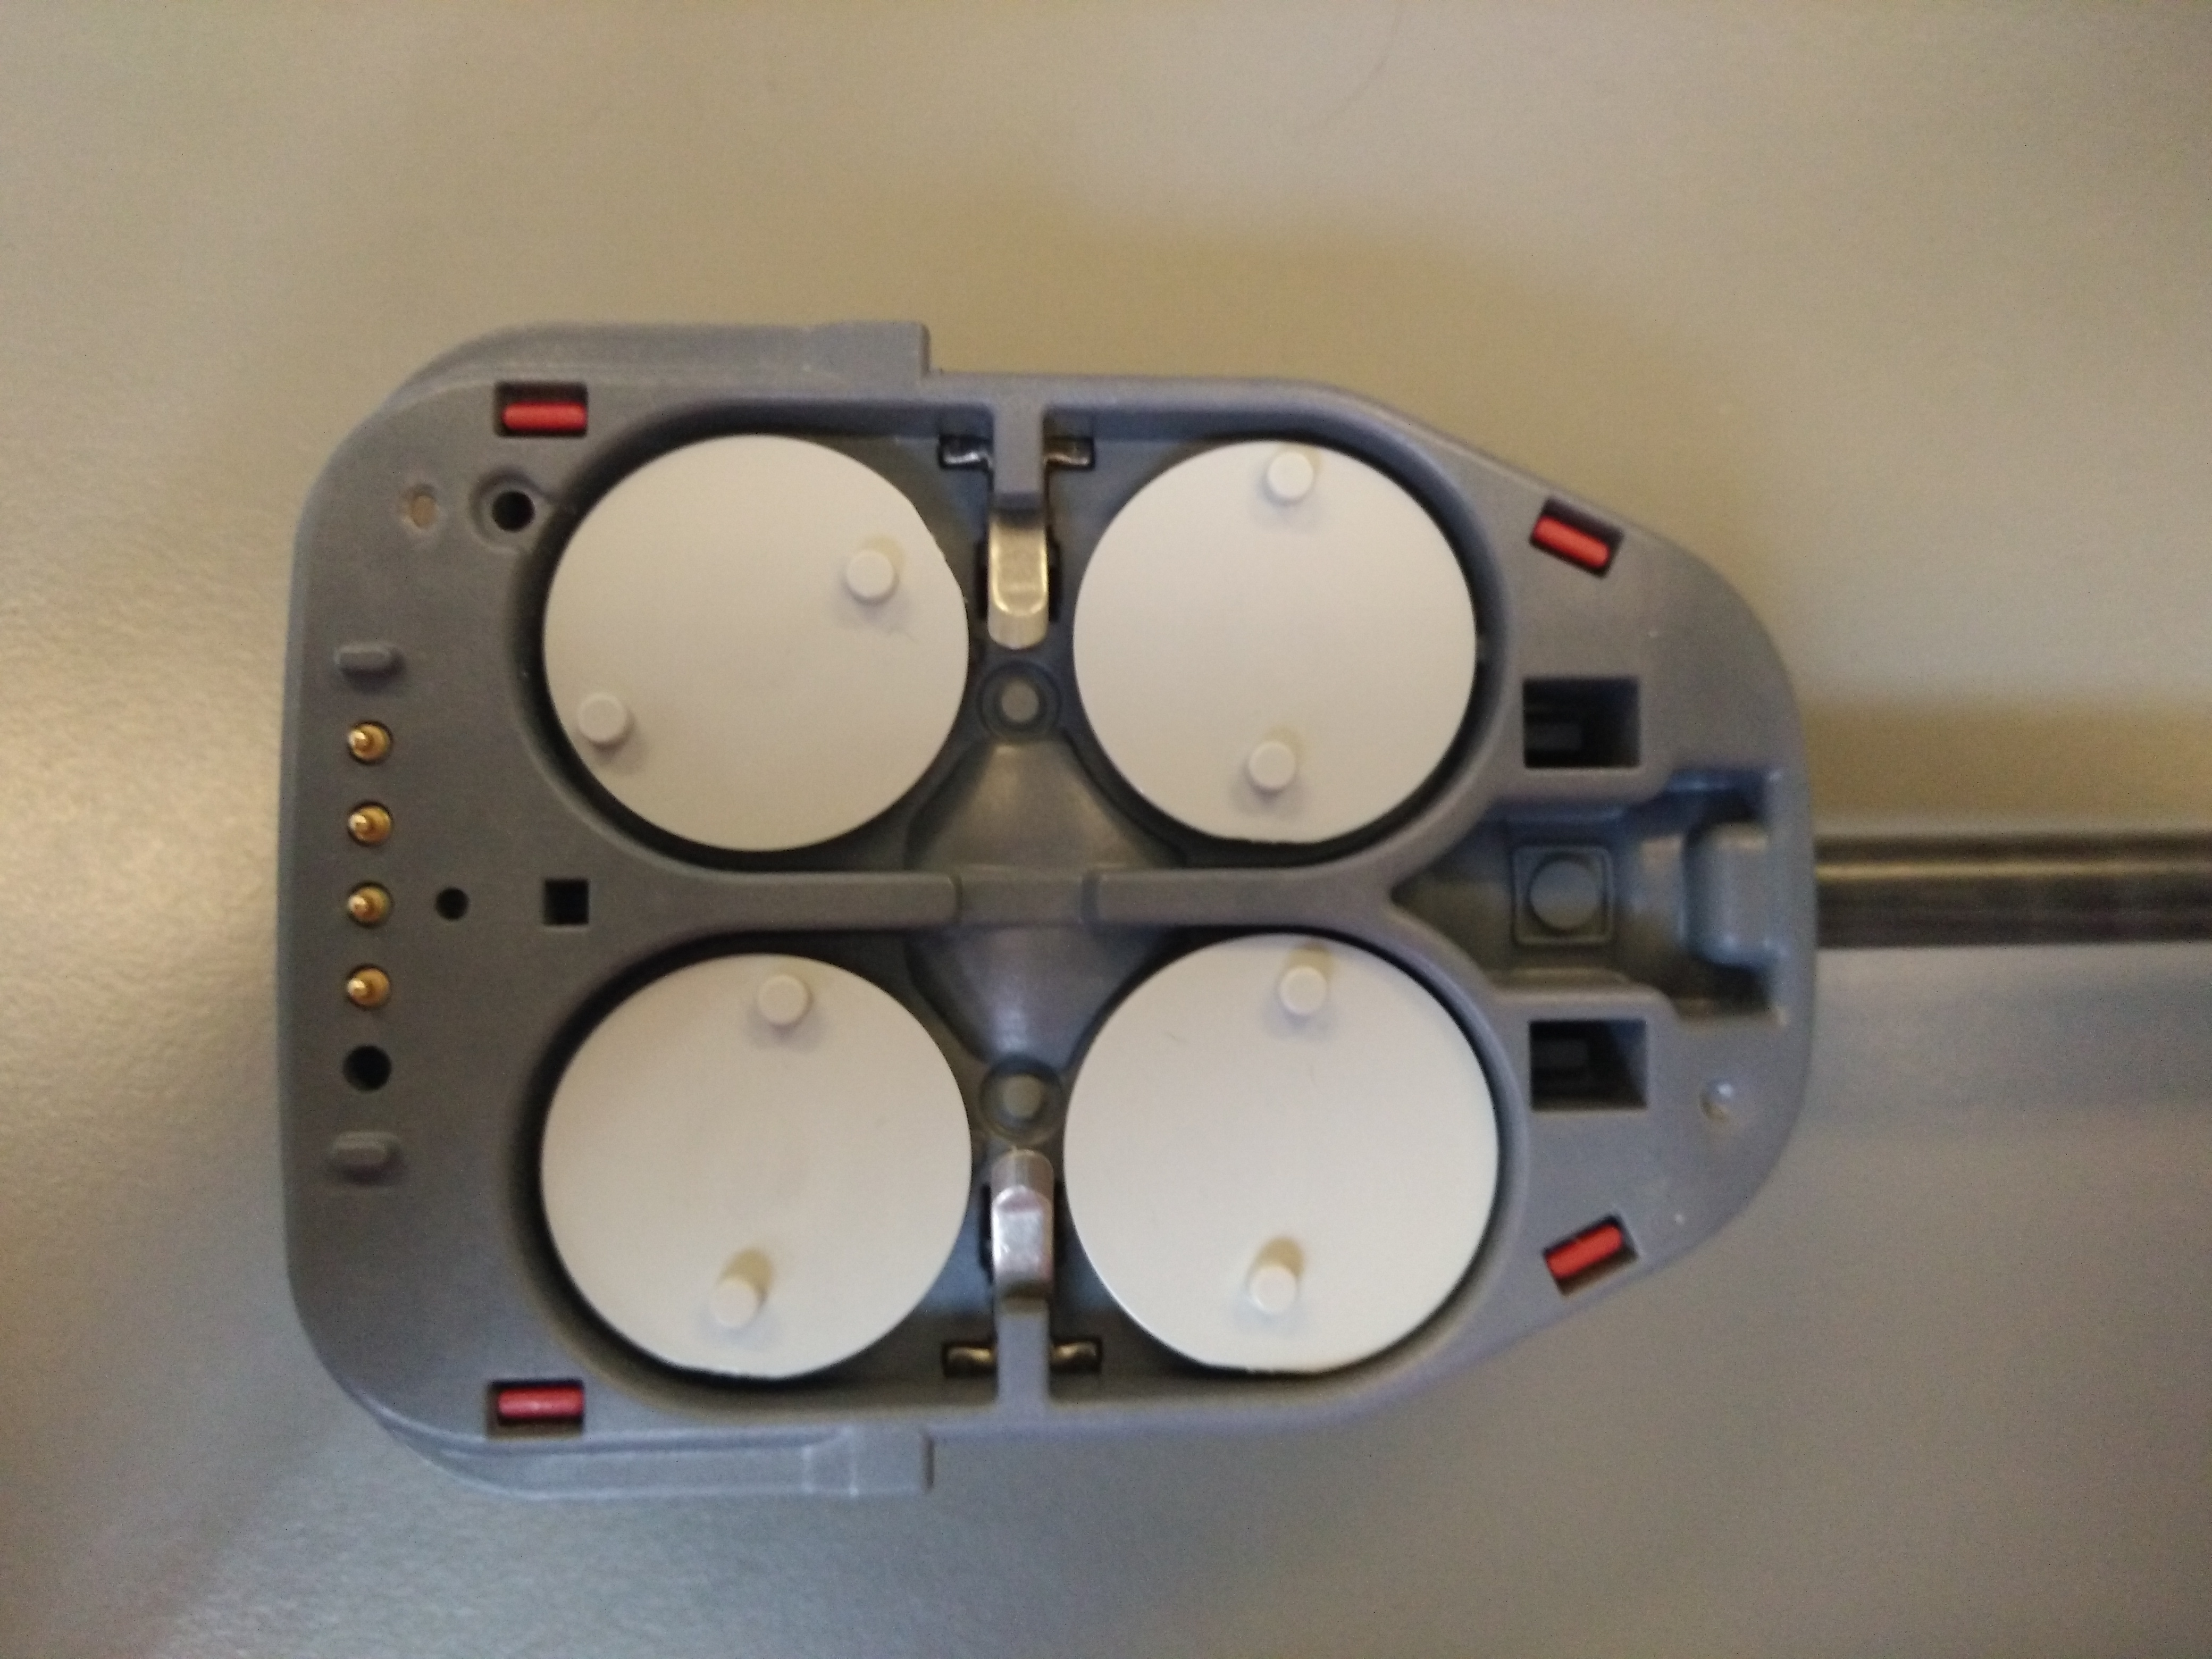
\includegraphics[width=\linewidth]{Endowrist2.jpg}
		\caption{Actuator plates, which can alternate the end effector position}
		\label{fig:Endo_plates}
	\end{subfigure}
	\begin{subfigure}{.32\textwidth}
		\centering
		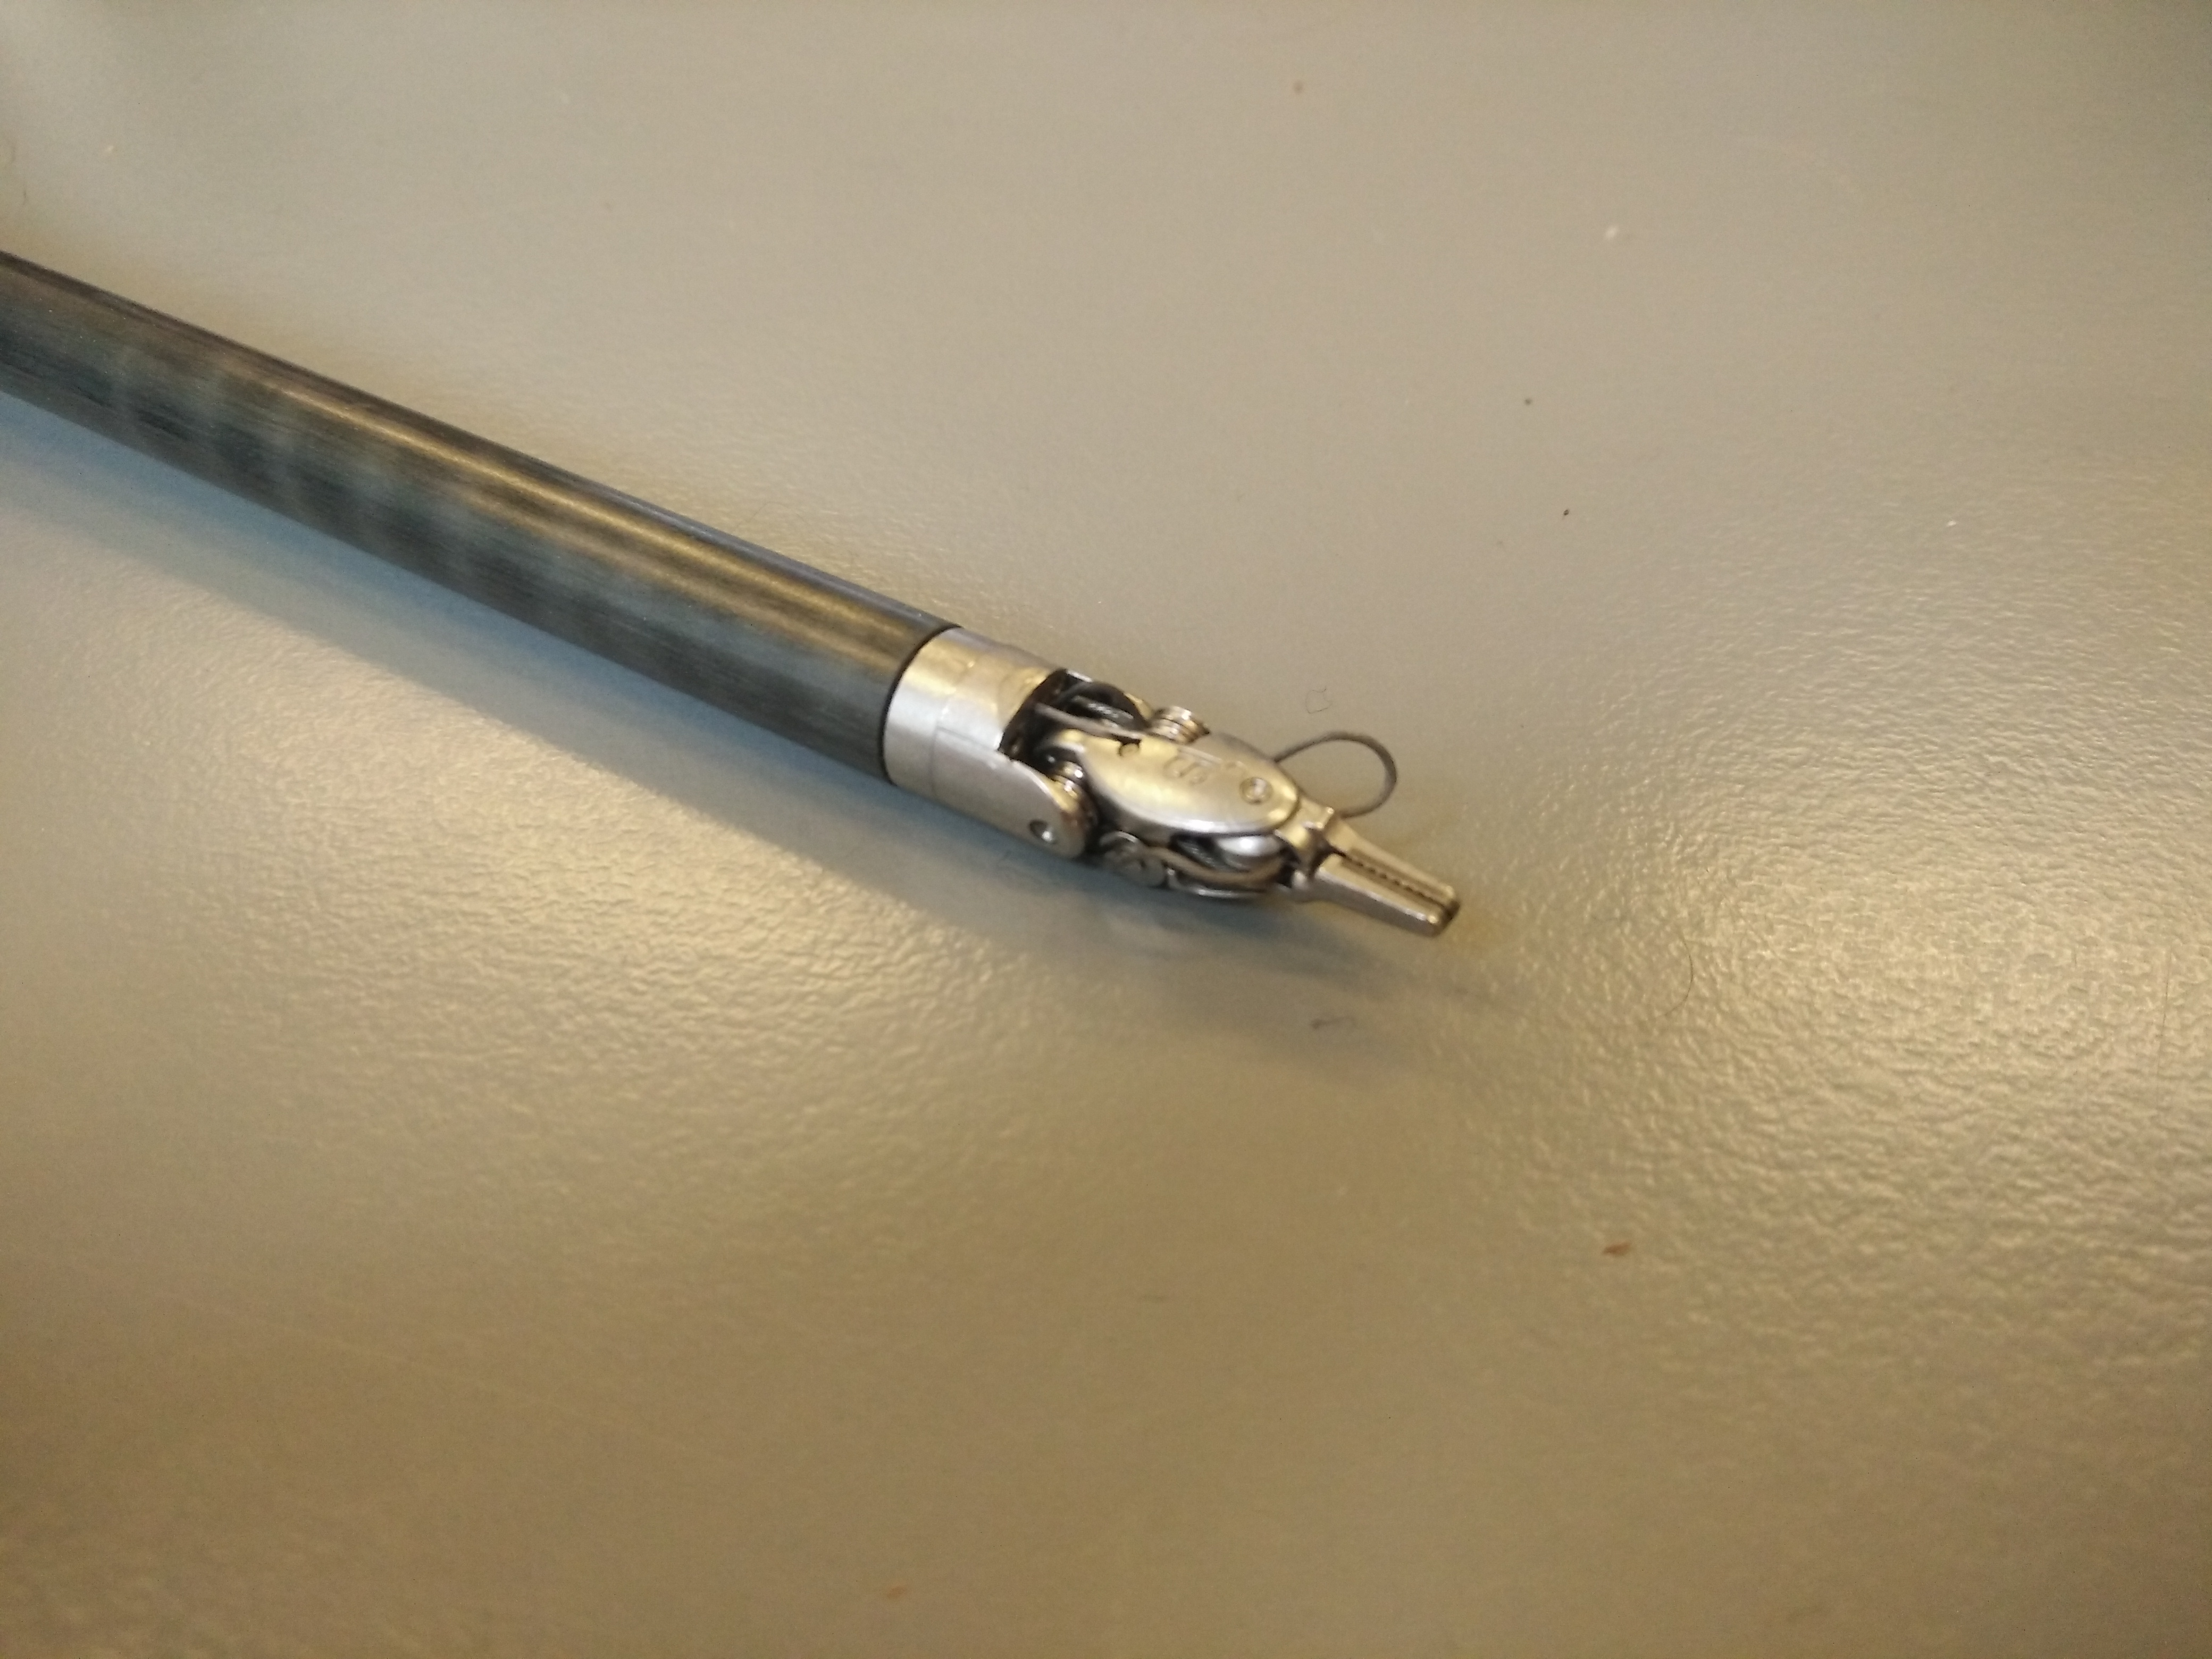
\includegraphics[width=\linewidth]{Endowrist3.jpg}
		\caption{End effector of the Endowrist\newline}
		\label{fig:Endo_end}
	\end{subfigure}
\caption{The Endowrist and how the interaction with it are made}
\label{fig:endowrits_set}
\end{figure}

As mentioned the Endowrist has the ability to be manipulated as a human wrist and thereby has four \gls{DOF}, see \figref{fig:Endo_end}.\todo{We have to update the picture so it shows each DOF}. This enables the movement of roll, pitch, yaw and an open closing mechanism that acts as the thumb and index finger of a hand. 

The end effector is manipulated by the four wheels seen on \figref{fig:Endo_plates}\todo{update with numbers}. Wheel one and three define the movement of the yaw and the closing mechanism. Wheel two and four moves the pitch and roll. The Endowrist is cable driven, which enables the opportunity of making the Endowrist small but it also makes the system nonlinear as the force acting at one end is not directly transmitted to the other end due to friction. 





\section{Mechanical test setup}\label{sec:Mechanical_testsetup.tex}
The mechanical test setup available at Aalborg University can be seen on \figref{fig:Mec_abcd}. It includes four of the motors described in \secref{Maxon_Motor} attached to the four rotational plates seen on \figref{fig:Mec_a} and \figref{fig:Mec_b}. These plates connect the motors and the Endowrist, such that the EndoWrist can be manipulated. See \figref{fig:Mec_c} and \figref{fig:Mec_d} for the attachment of the Endowrist to the EndoWrist holder.  

\begin{figure}[H]
	\centering
	\begin{minipage}[t]{0.9\textwidth}
	\begin{subfigure}{0.45\textwidth}
		\vspace{-10pt}
		\centering
		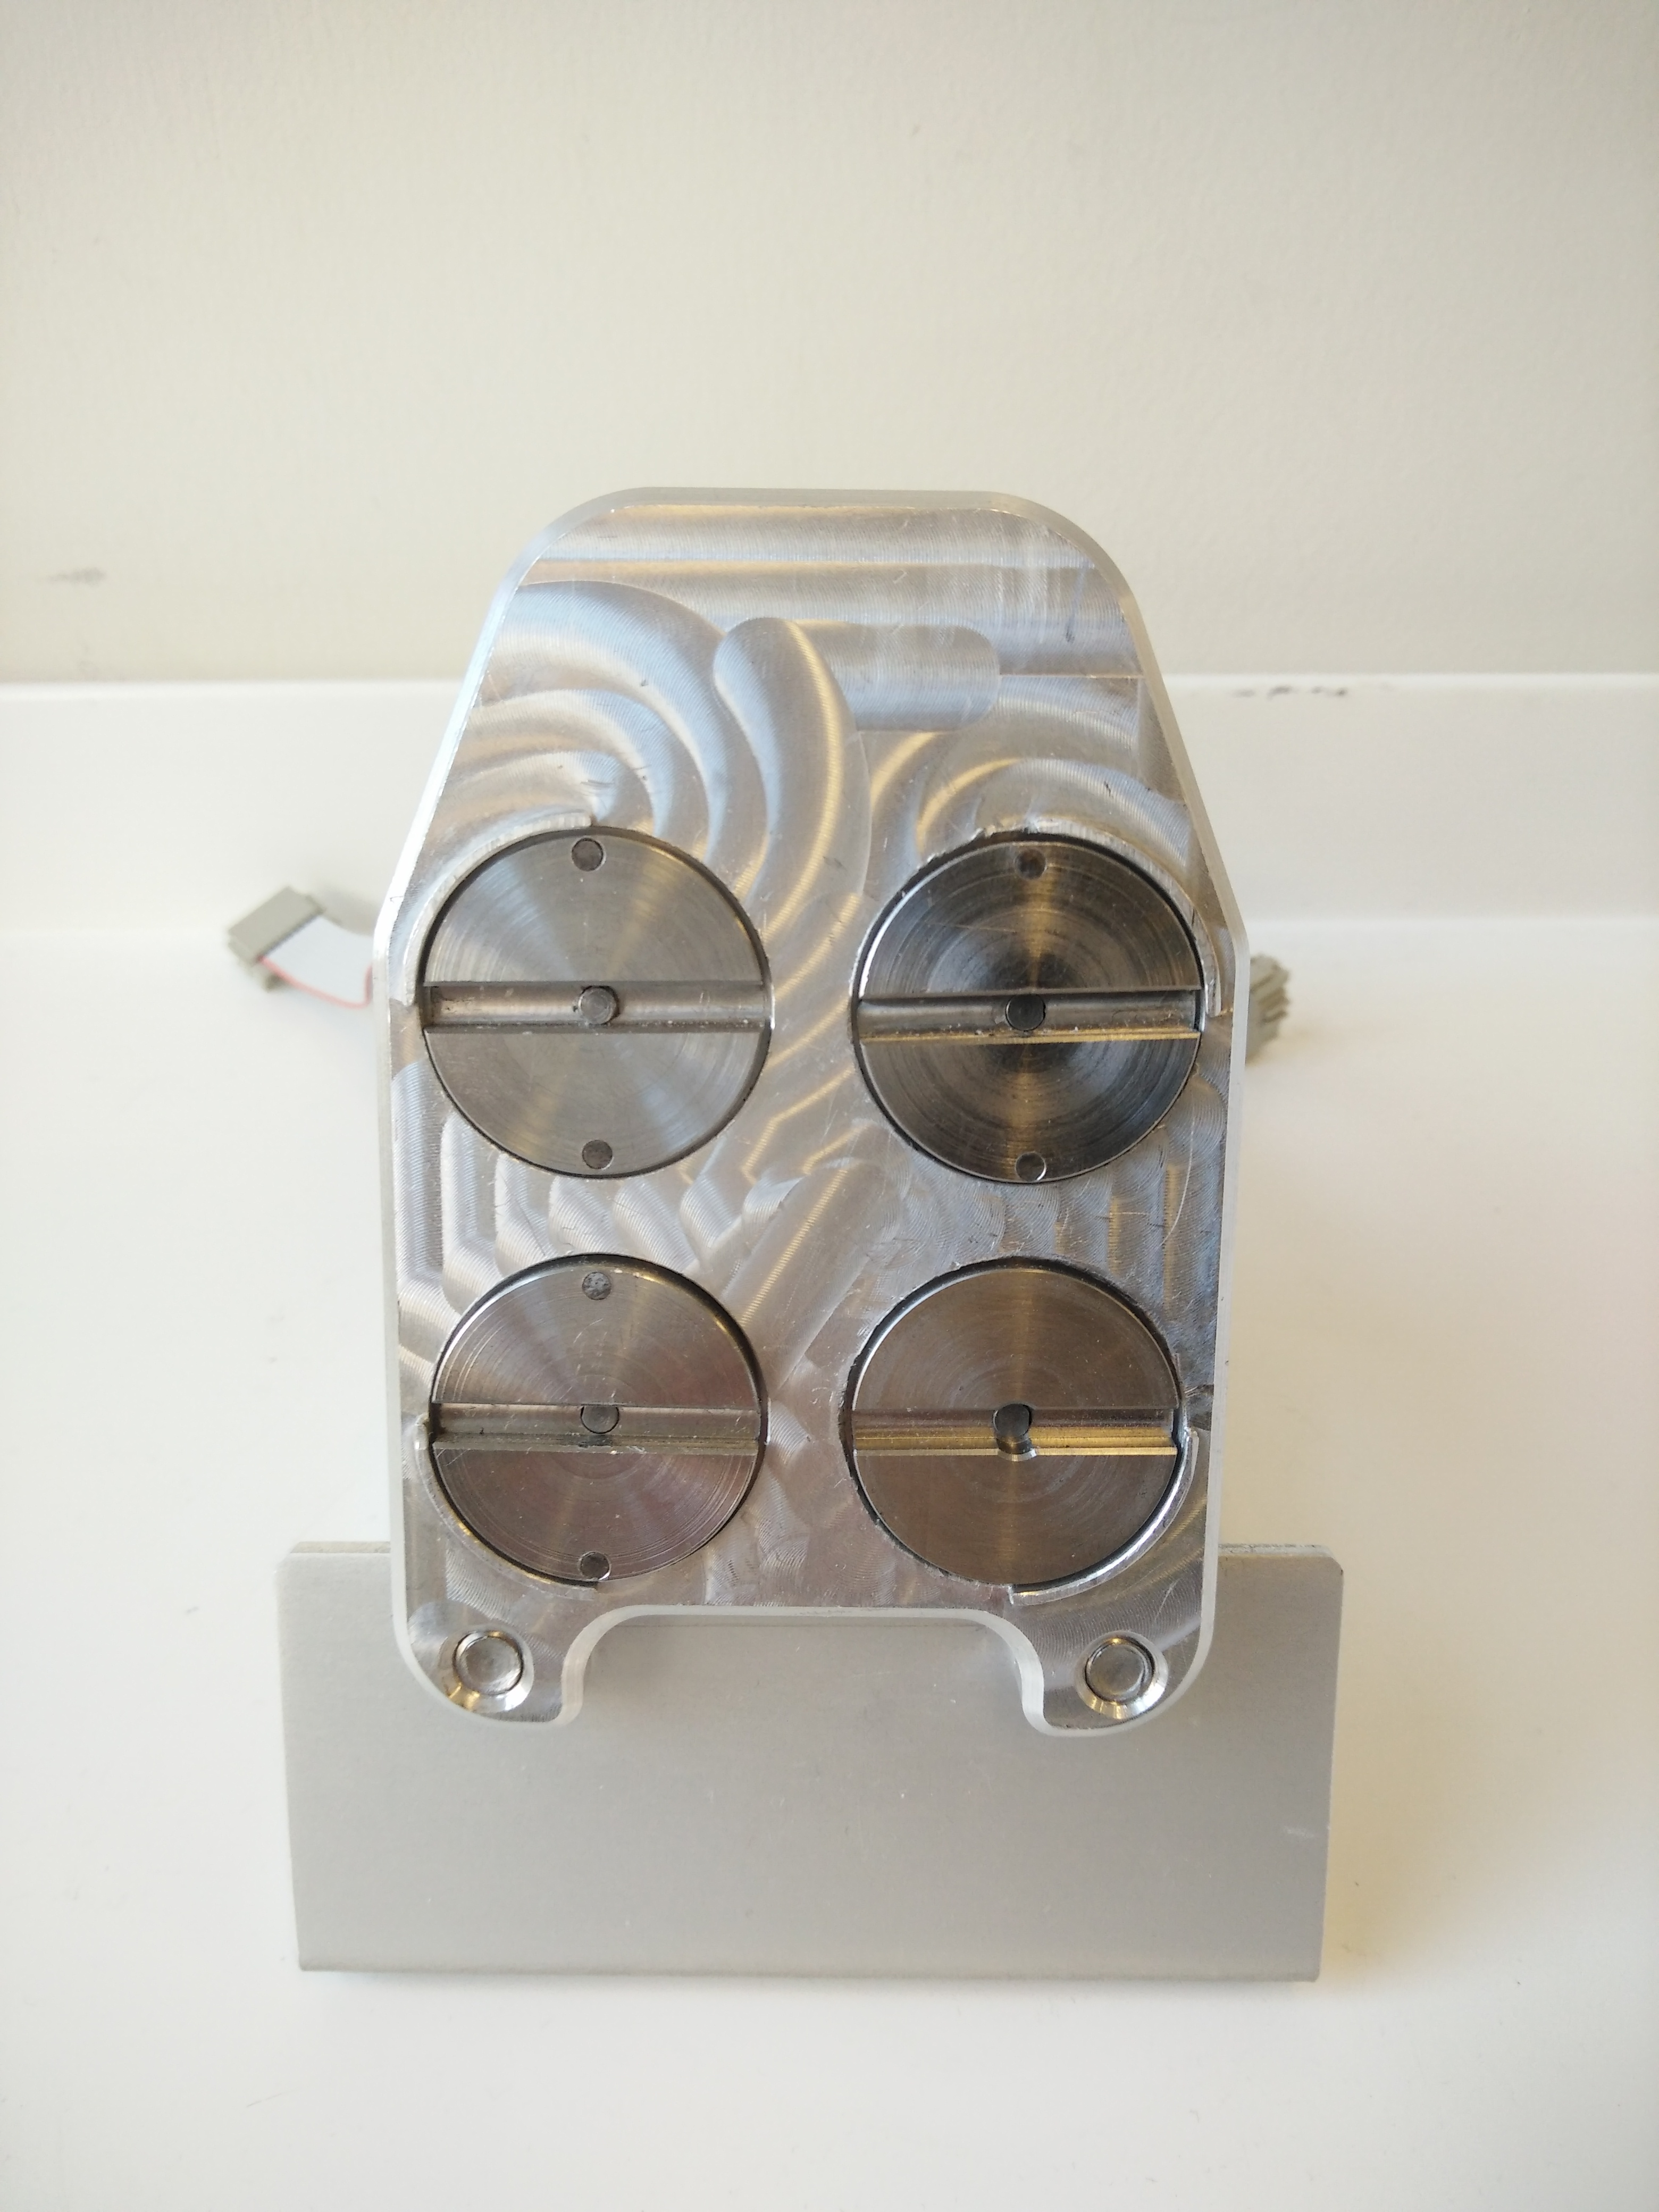
\includegraphics[width=\linewidth]{Test_setup1.jpg}
		\caption{EndoWrist holder. Front view}
		\label{fig:Mec_a}
	\end{subfigure}
	\hspace{\fill}
	\begin{subfigure}{0.45\textwidth}
		\centering
		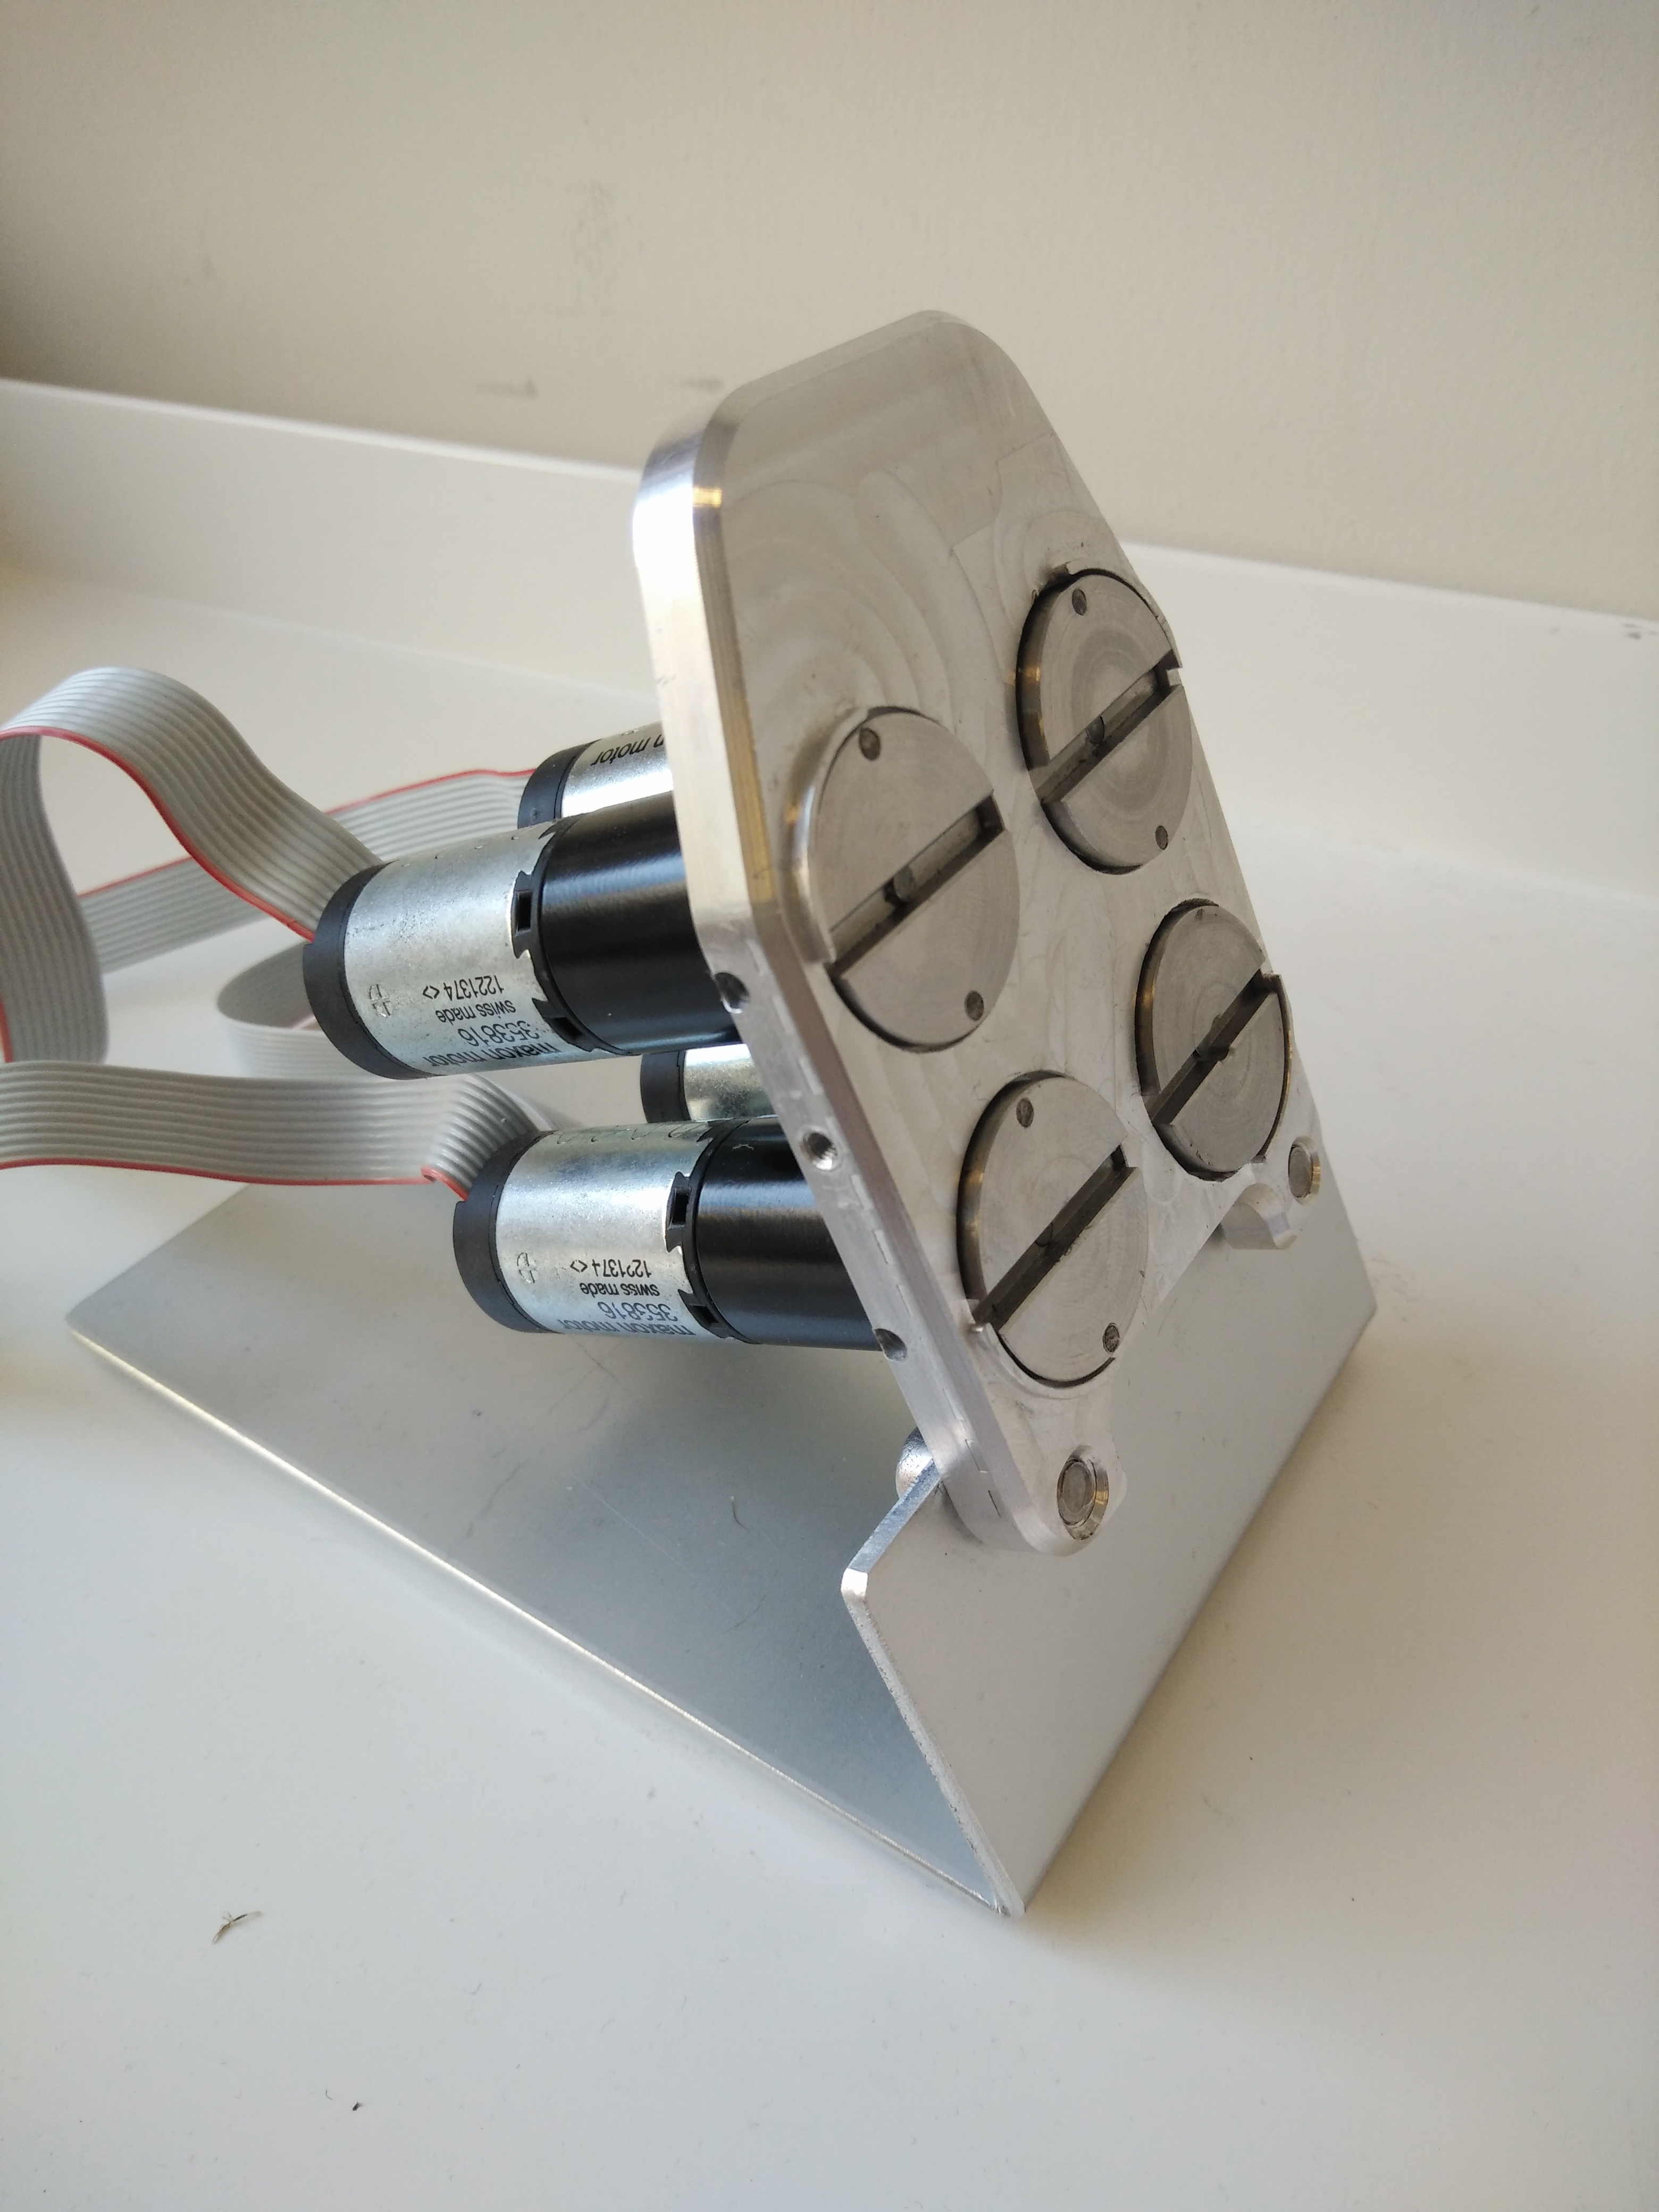
\includegraphics[width=\linewidth]{Test_setup2.jpg}
		\caption{EndoWrist holder with motors at the back. Side view}
		\label{fig:Mec_b}
	\end{subfigure}
	\end{minipage}

	\begin{minipage}[t]{0.9\textwidth}
	\vspace{20pt}
	\begin{subfigure}{0.45\textwidth}
		\vspace{0pt}
		\centering
		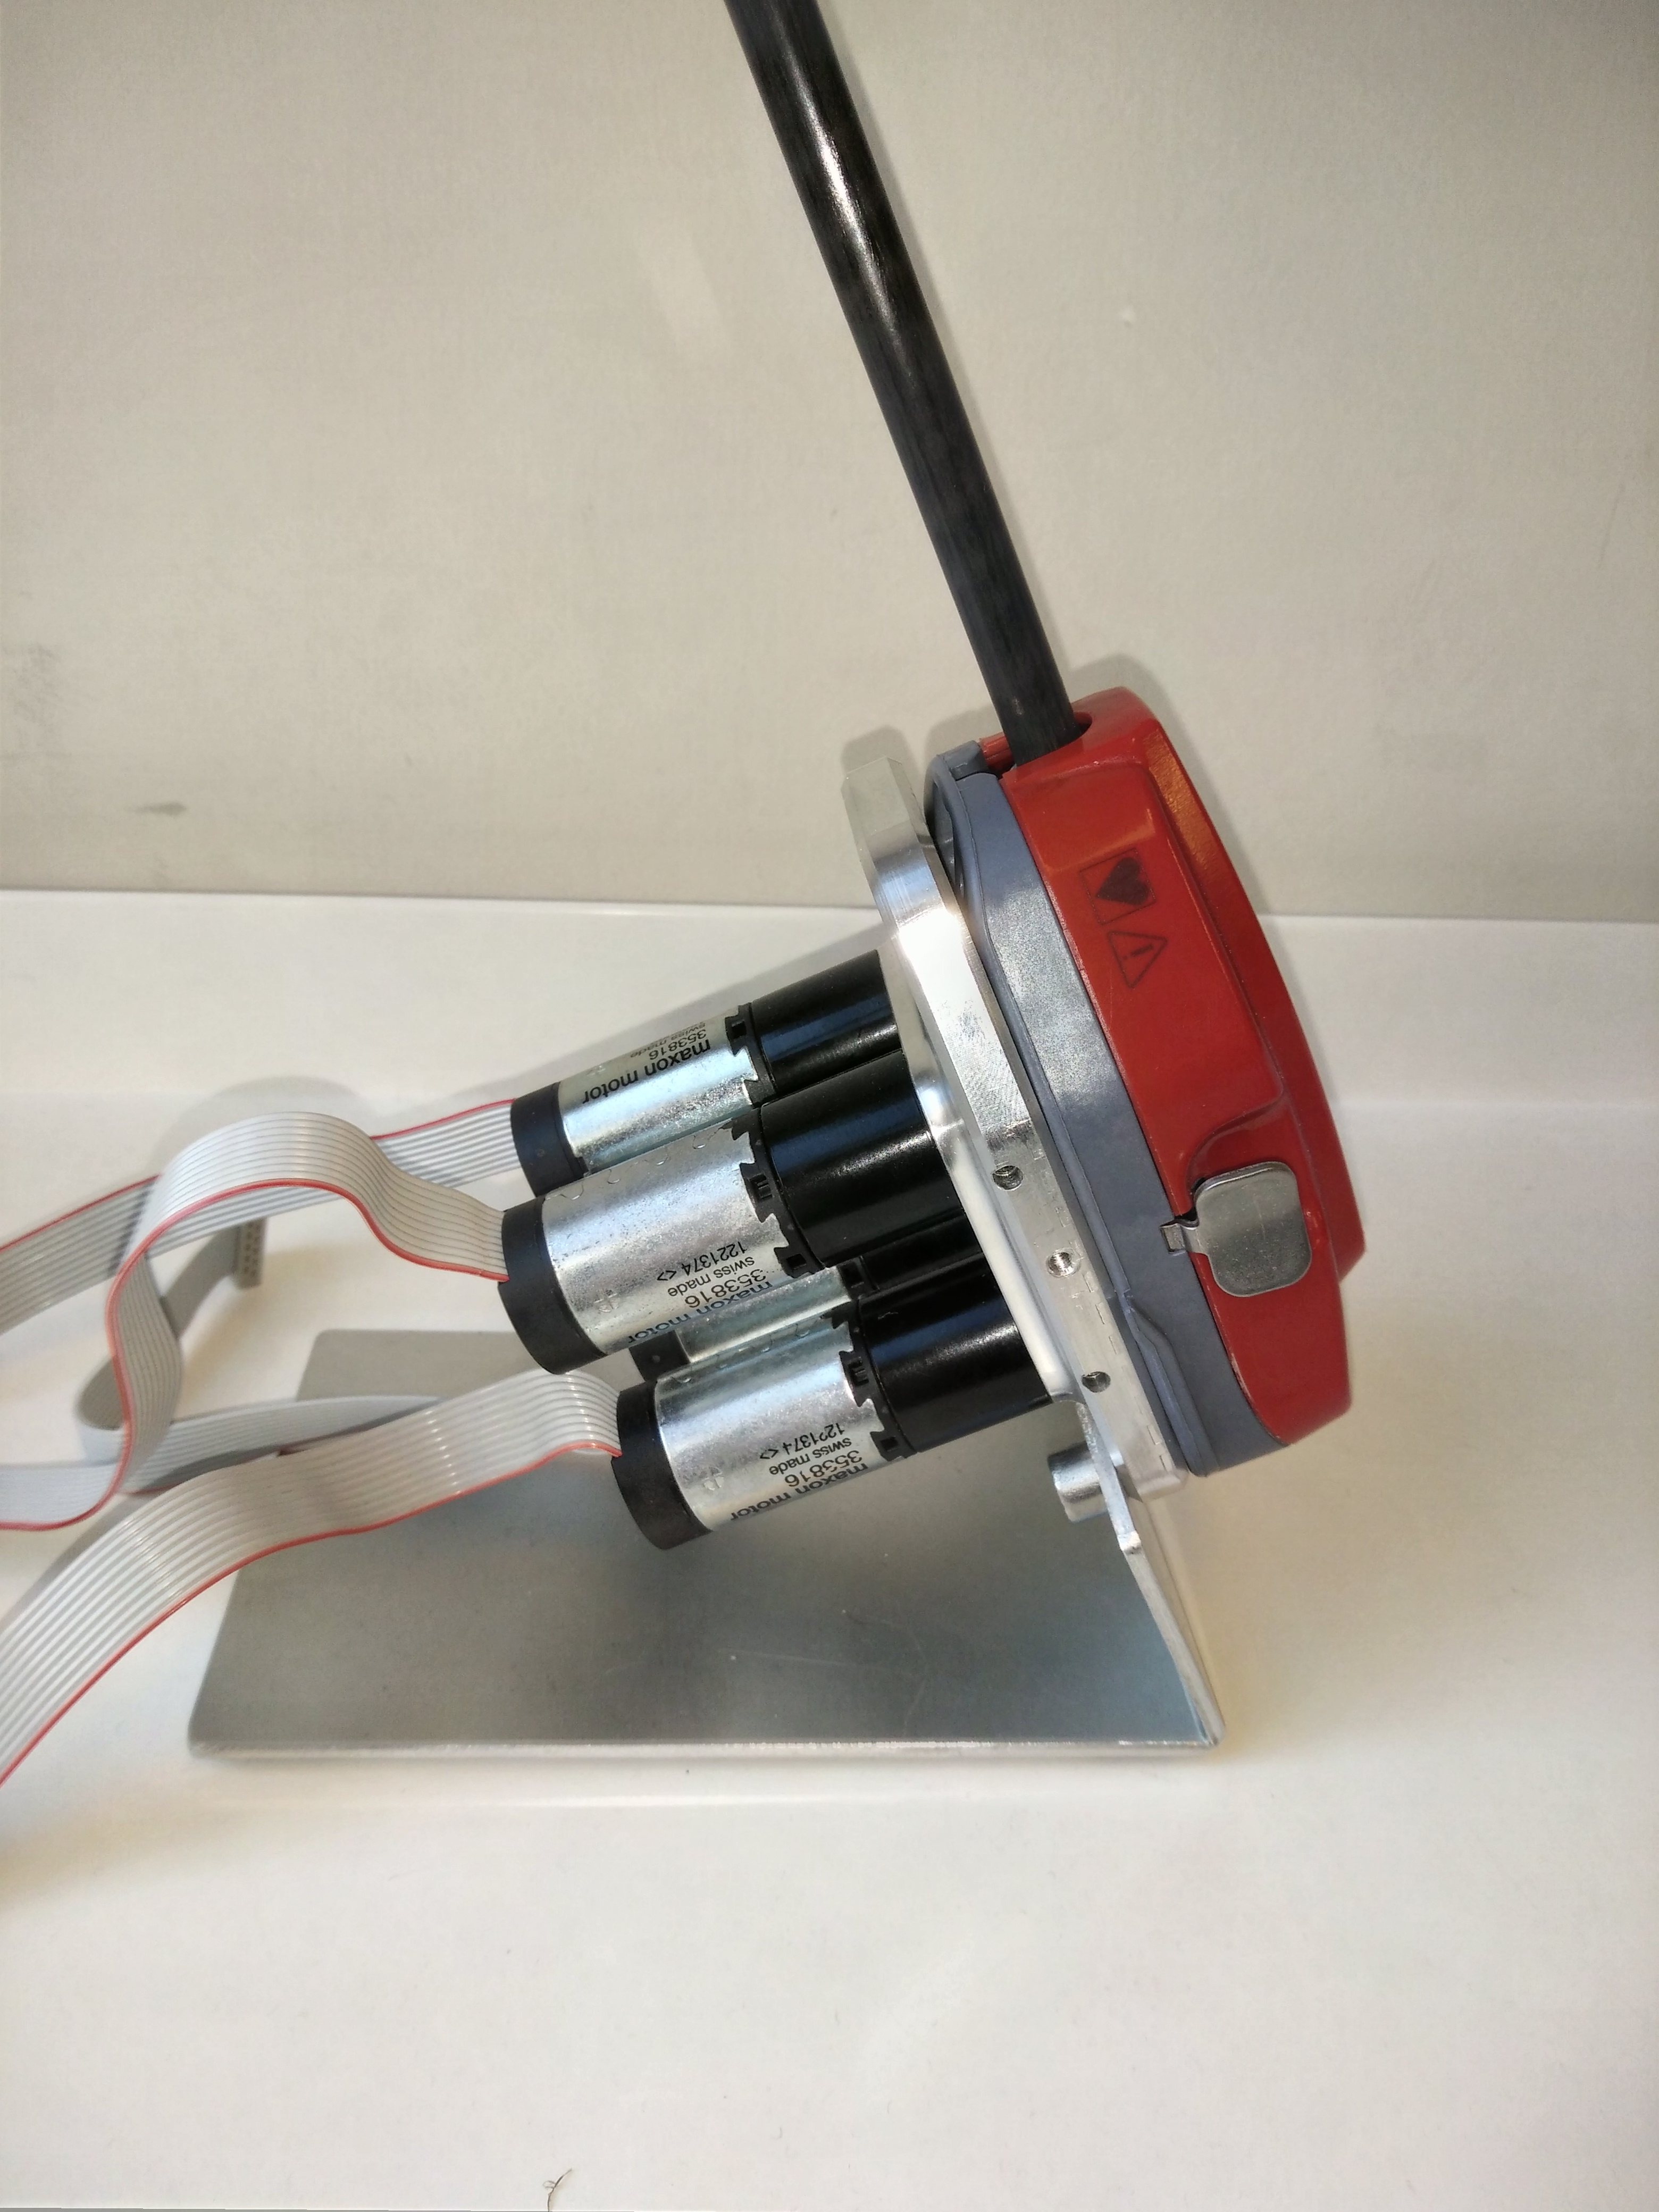
\includegraphics[width=\linewidth]{Test_setup3.jpg}
		\caption{EndoWrist holder with EndoWrist and motors. Side view}
		\label{fig:Mec_c}
	\end{subfigure}
	\hspace{\fill}
	\begin{subfigure}{0.45\textwidth}
		\centering
		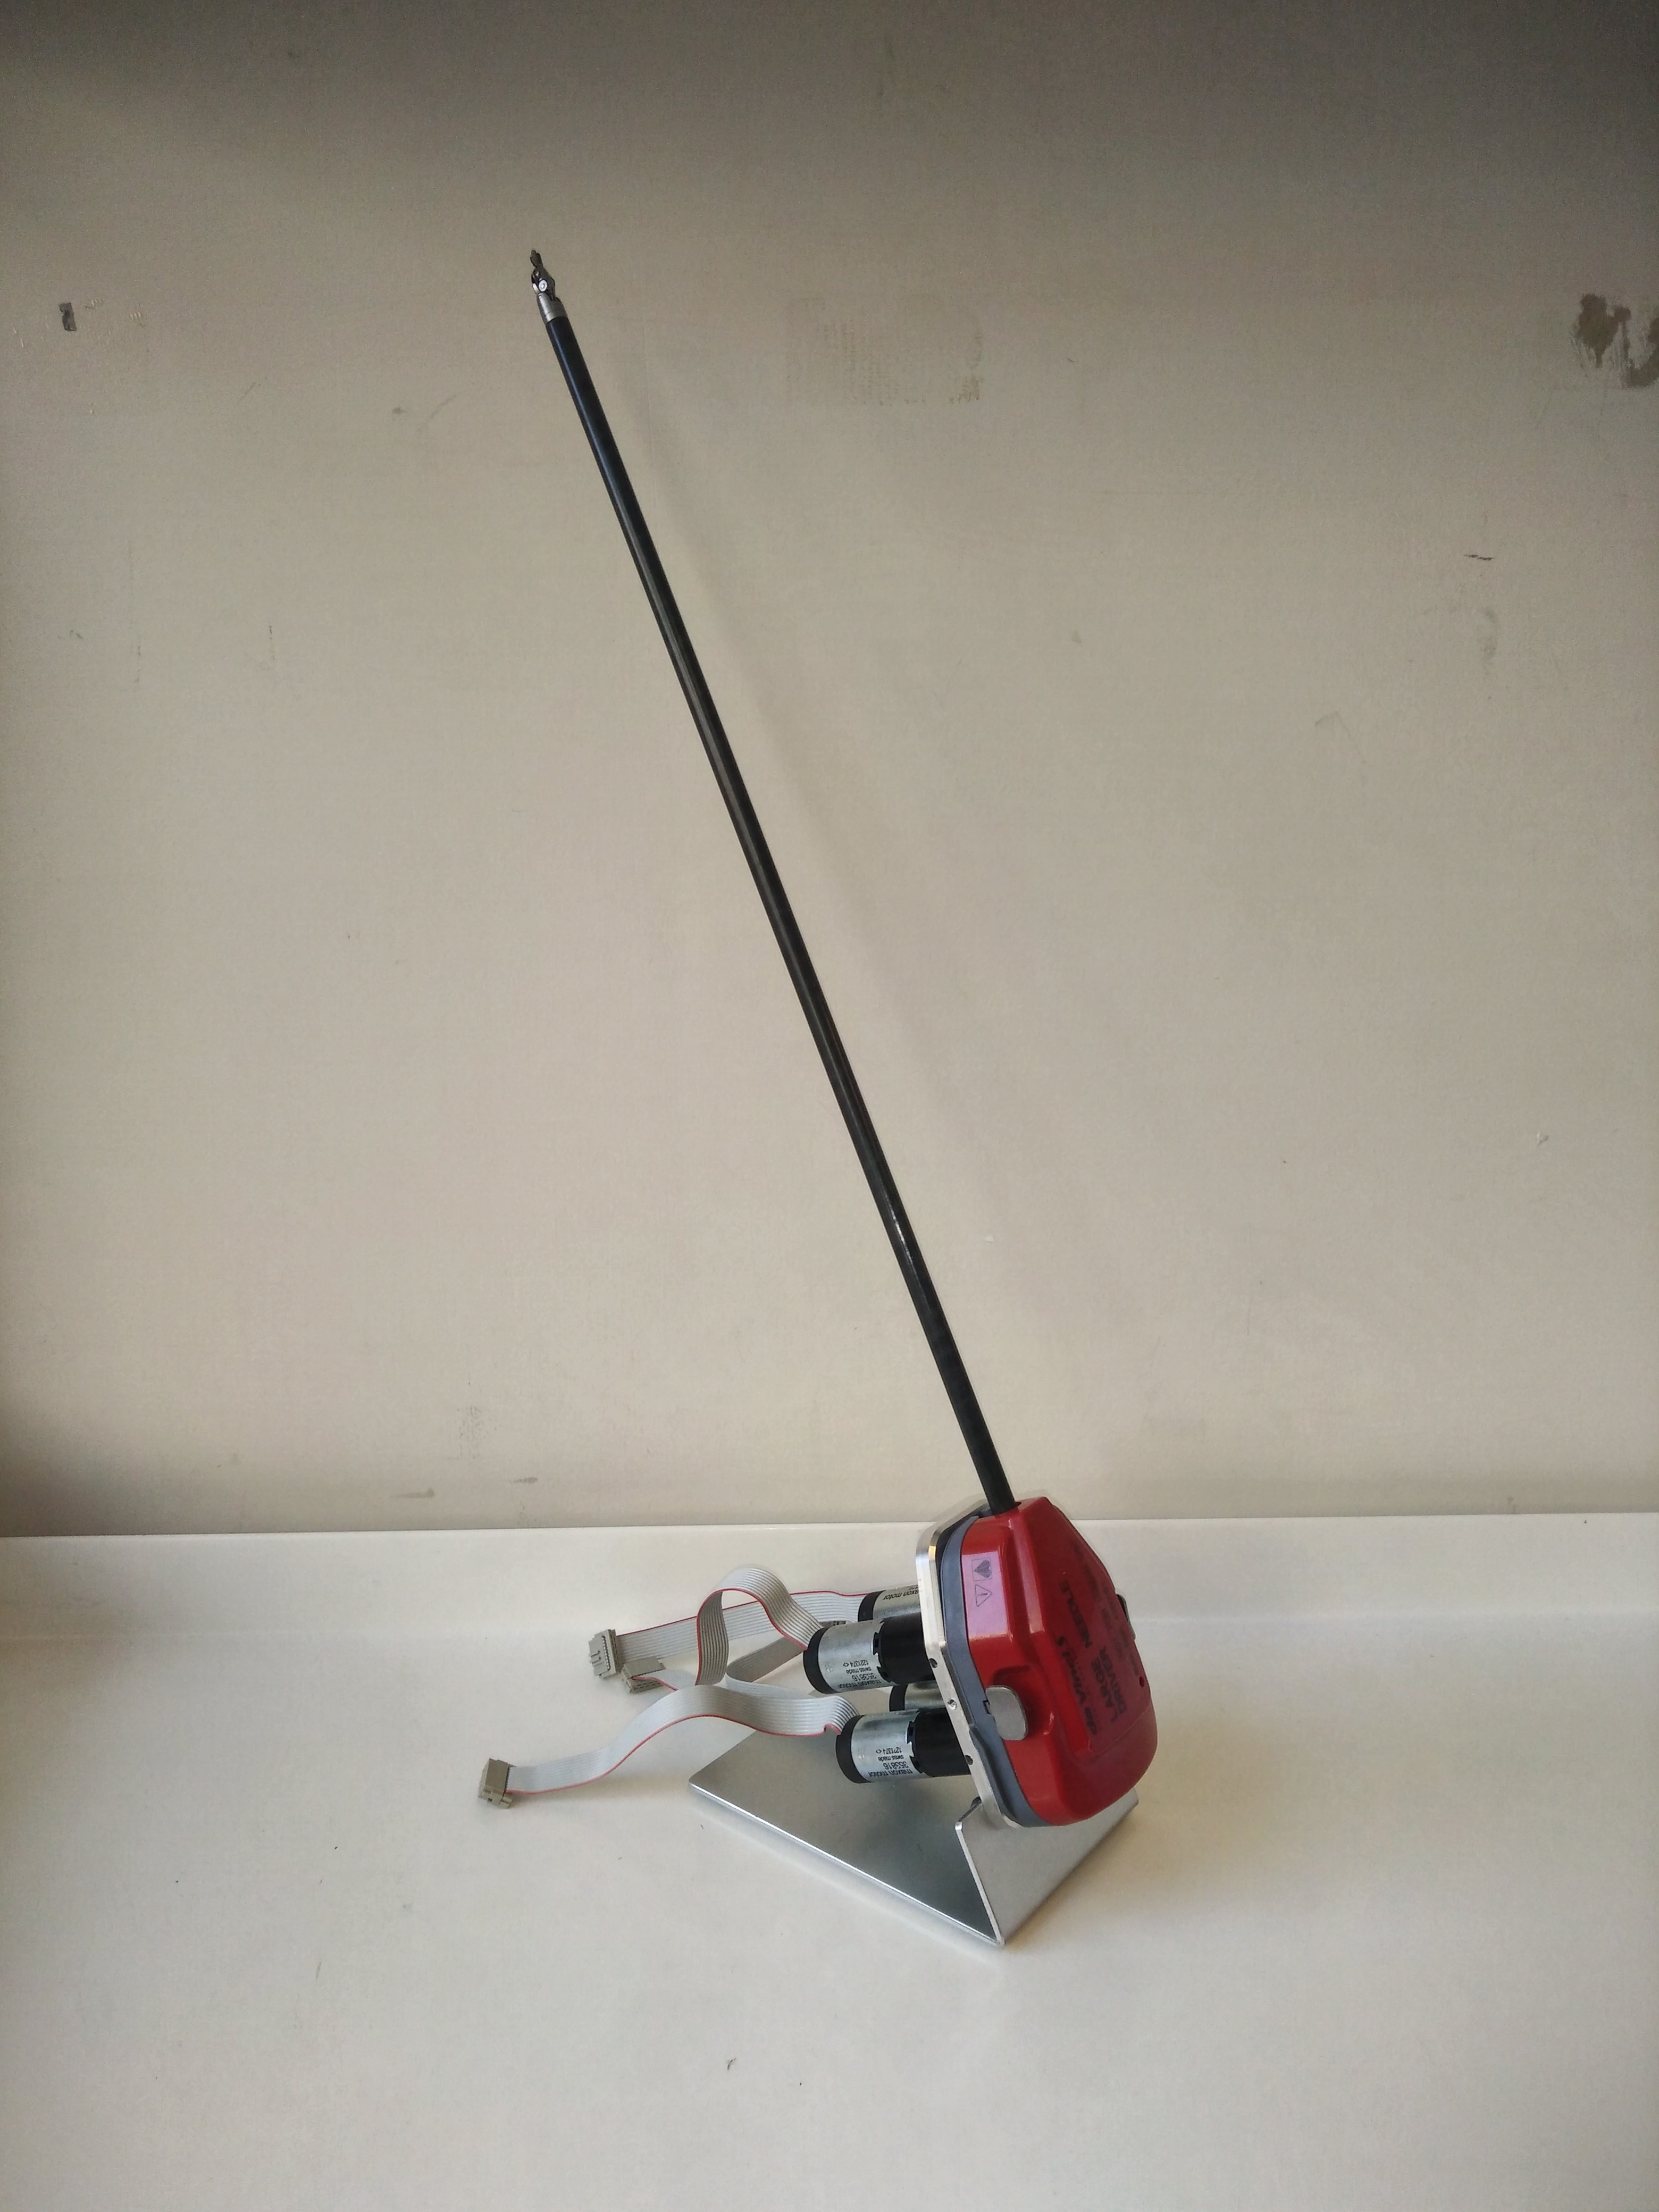
\includegraphics[width=\linewidth]{Test_setup4.jpg}
		\caption{Full view of the mechanical test setup}
		\label{fig:Mec_d}
	\end{subfigure}
	\end{minipage}

	\caption{Four pictures of the mechanical test setup available at Aalborg University, which include motors, EndoWrist and EndoWrist holder}
	\label{fig:Mec_abcd}
\end{figure}

This setup can manipulate the EndoWrist in the same manner as if the tool was connected to the da Vinci robot, see \secref{sec:da_vin_rob}.
\todo{Does this last line explaine what the setup can do in a proper manner?}

\section{Motor}\label{Maxon_Motor}
The four motors actuating the EndoWrist is sold as a bulk solution which include motor\cite{motor_motor}, gear\cite{motor_gear} and a position encoder\cite{motor_encoder}, see \figref{fig:Full_motor _dis}.
These motors are direct current (DC) motors. The main parameters for this bulk solution are listed below:

\begin{itemize}
	\item Torque constant: $10.9\frac{\text{mNm}}{\text{A}}$
	\item Nominal continues current: 0.681 A 
	\item Gearing ratio: 1:19
	\item Encoder precision: 512 counts pr. rotation. With the proper programming, see section \ref{encount}, 2048 positions can be distinguished in one rotation.
\end{itemize}

\begin{figure}[H]
	\centering
	\begin{subfigure}{.32\textwidth}
		\vspace{0pt}
		\centering
		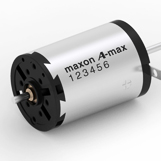
\includegraphics[width=\linewidth]{motor.jpg}
		\caption{The Maxon 110160 \newline DC motor.}
		\label{fig:motor}
	\end{subfigure}
	\begin{subfigure}{.32\textwidth}
		\centering
		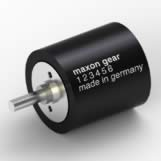
\includegraphics[width=\linewidth]{motor_gear.jpg}
		\caption{The planetary gearhead, 110356, equipped with sleeve bearing.}
		\label{fig:motor_gear}
	\end{subfigure}
	\begin{subfigure}{.32\textwidth}
		\hspace{5pt}
		\centering
		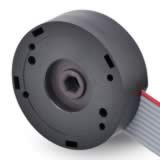
\includegraphics[width=\linewidth]{motor_sensor.jpg}
		\caption{The encoder, 201937, used for getting angular data.}
		\label{fig:motor_sensor}
	\end{subfigure}
	\caption{The combination gear disassembled}
	\label{fig:Full_motor _dis}
\end{figure}

The control of these motors are done through the ESCON controller boards, connected to the sbRIO, as shown on \figref{interface}. A detailed description is provided in \secref{sec:motor_control}.

% \begin{figure}[H]
% \centering
% \begin{tikzpicture}
% %\draw (-1.5,-1.5) rectangle (13.5,1.5);

% \draw (-2.8,3.1) rectangle (2.8,-12.8);
% \node at (0,2.5) {\textbf{sbRIO}};


% \draw (-2.5,2) rectangle (2.5,-4.2);
% \node at (0,1.5) {\textbf{Micro processor}};
% \node[box] (datlog) at (0,0.3) {Data logging};
% \node[box] (ethcommu) at ($(0,-1.7) + (datlog)$) {Ethernet communication};
% \node[box] (shuterr) at ($(0,-1.7) + (ethcommu)$) {Shutdown:\\Communication error};


% \draw (-2.5,-4.7) rectangle (2.5,-12.6);
% \node at (0,-5.2) {\textbf{FPGA}};
% \node[box] (poscon) at ($(0,-3.3) + (shuterr)$) {Position control};
% \node[box] (enco) at ($(0,-1.7) + (poscon)$) {Encoder counter};
% \node[box] (PWM) at ($(0,-1.7) + (enco)$) {PWM control};
% \node[box] (dataES) at ($(0,-1.7) + (PWM)$) {Read data: ESCON};


% \draw (-9,-6) rectangle (-4,-12.6);
% \node[box] (spcon) at (-6.5,-8) {Speed control\\with inner current\\control};
% \node at ($(spcon) + (0,1.5)$) {\textbf{ESCON}};
% \node at ($(spcon) + (0,1.2)$) {\textbf{motor controller}};
% \node[box] (limcu) at ($(0,-1.7) + (spcon)$) {Limit output\\current};
% \node[box] (reen) at ($(0,-1.7) + (limcu)$) {Read encoder\\ticks};


% \draw (-9,-5.5) rectangle (-4,-4);
% \node at (-6.5,-4.75) {\textbf{Motor}};


% \draw (-9,-3.5) rectangle (-4,3.1);
% \node at (-6.5,2.5) {\textbf{ROS computer}};

%\node[fill = {rgb:red,1;green,2;blue,5},box] (Opt) at (0,0) {Operator};
%\node[fill = {rgb:red,1;green,2;blue,5},box] (Geo) at ($(3,0) + (Opt)$) {};
%\node[fill = {rgb:red,1;green,2;blue,5},box] (ros) at ($(3,0) + (Geo)$) {Robotic\\operating\\system};
%\node[fill = {rgb:red,1;green,2;blue,5},box] (davin) at ($(3,0) + (ros)$) {Da Vinci\\robot};
%\node[fill = {rgb:red,1;green,2;blue,5},box] (end) at ($(3,0) + (davin)$) {Endowrist};


%\draw[->, ultra thick] ([yshift=0.3cm]Opt.east) -- ([yshift=0.3cm]Geo.west);
%\draw[->, ultra thick] ([yshift=0.3cm]Geo.east) -- ([yshift=0.3cm]ros.west);
%\draw[->, ultra thick] ([yshift=0.3cm]ros.east) -- ([yshift=0.3cm]davin.west);
%\draw[->, ultra thick] ([yshift=0.3cm]davin.east) -- ([yshift=0.3cm]end.west);


%\draw[<-, ultra thick] ([yshift=-0.3cm]Opt.east) -- ([yshift=-0.3cm]Geo.west);
%\draw[<-, ultra thick] ([yshift=-0.3cm]Geo.east) -- ([yshift=-0.3cm]ros.west);
%\draw[<-, ultra thick] ([yshift=-0.3cm]ros.east) -- ([yshift=-0.3cm]davin.west);
%\draw[<-, ultra thick] ([yshift=-0.3cm]davin.east) -- ([yshift=-0.3cm]end.west);

%\node at (1.5,1) {Position};
% \node at (4.5,1) {Position};
% \node at (7.5,1) {yes};
% \node at (10.5,1) {yes};

%\node at (1.5,-1) {Force};
% \node at (4.5,1) {Position};
% \node at (7.5,1) {yes};
% \node at (10.5,1) {yes};
%\end{tikzpicture}
%\caption{Overall system with feedback in both direction}
%\end{figure}



\begin{figure}[H]
\centering
\tikzset{dataset/.style = {rectangle, draw, text width = 5.5cm, minimum height=3cm}}
\begin{tikzpicture}

\node [dataset] (mpro) at (0,3) {\textbf{Micro processor}
\begin{itemize}[itemsep=0pt,partopsep=0pt,topsep=0pt]
\item Data logging
\item Ethernet communication
\item Shutdown: Communication error \\
\end{itemize}};

\node [dataset, below of=mpro, node distance=6.5cm] (FPGA) {\textbf{FPGA}
\begin{itemize}[itemsep=0pt,partopsep=0pt,topsep=0pt] 
\item Position contron
\item Encoder counter
\item PWM control
\item Read data: Escon 
\end{itemize}};

\draw[->, ultra thick] ([xshift=-1cm]mpro.south) -- ([xshift=-1cm]FPGA.north);
\draw[<-, ultra thick] ([xshift=1cm]mpro.south) -- ([xshift=1cm]FPGA.north);

\node [dataset, left of=FPGA, node distance=7cm] (emc) {\textbf{ESCON motor controller}
\begin{itemize}[itemsep=0pt,partopsep=0pt,topsep=0pt] 
\item Speed controll with intter current control
\item Limit output current
\item Read encoder ticks 
\end{itemize}};

\draw[->, ultra thick] ([yshift=-1cm]emc.east) -- ([yshift=-1cm]FPGA.west);
\draw[<-, ultra thick] ([yshift=1cm]emc.east) -- ([yshift=1cm]FPGA.west);

\tikzset{dataset/.style = {rectangle, draw, text width = 6cm, minimum height=10.5cm}}
\node [dataset, above of=FPGA, node distance=3.5cm] (motor) {\textbf{sbRIO}
\begin{itemize}[itemsep=0pt,partopsep=0pt,topsep=260pt] % Edit the last number to fit title 
\item[]  %  This line is necessary!!
\end{itemize}};


\tikzset{dataset/.style = {rectangle, draw, text width = 5.5cm, minimum height=1cm}}
\node [dataset, above of=emc, node distance=2.5cm] (motor) {\textbf{Motor}};

\draw[->, ultra thick] ([xshift=-1cm]motor.south) -- ([xshift=-1cm]emc.north);
\draw[<-, ultra thick] ([xshift=1cm]motor.south) -- ([xshift=1cm]emc.north);

\tikzset{dataset/.style = {rectangle, draw, text width = 5.5cm, minimum height=5cm}} % This edits the size of the Ros computer box 
\node [dataset, above of=motor, node distance=3.75cm] (ROS) {\textbf{Ros computer}
\begin{itemize}[itemsep=0pt,partopsep=0pt,topsep=0pt] 
\item 1
\item 2
\item 3 
\end{itemize}};

\draw[->, ultra thick] ([yshift=-1cm]mpro.west) -- ([yshift=-1cm]ROS.east); % ([yshift=-1cm]ROS.west) should probaly be edited!!!
\draw[<-, ultra thick] ([yshift=1cm]mpro.west) -- ([yshift=1cm]ROS.east);

% \draw [->,ultra thick] (-1,1.5) -- (-1,-2); %Micro to FPGA
% \draw [<-,ultra thick] (1,1.5) -- (1,-2);

% \draw [->,ultra thick] (-3,-3) -- (-4,-3);
% \draw [<-,ultra thick] (-3,-4) -- (-4,-4);

\end{tikzpicture}
\caption{Say somthing cool- "\textit{Somthing cool!}"}
\end{figure}

\todo{Include arrow, label anc new caption... elaborate this picture breifly, what do the different boxes do?}

% \begin{figure}[htb]
% \tikzset{dataset/.style = {rectangle, draw, text width = 5cm, minimum height=1in}}
% \begin{tikzpicture}[auto, font={\scriptsize}]
%     % Place nodes
%     \node [dataset] (tm) {Data 1 
%                             \begin{itemize}[itemsep=0pt,partopsep=0pt,topsep=0pt]   %% this added.
%                                 \item{\# Adults } 
%                                 \item{\# Children} 
%                                 \item{Income}
%                                 \item{Ethnicity}
%                             \end{itemize}\par};
%     \node [dataset, right of=tm, node distance=3in] (dmv) {Data 2 
%                             \begin{itemize}[itemsep=0pt,partopsep=0pt,topsep=0pt] 
%                                 \item{Data 2} 
%                             \end{itemize}\par};
%     % draw links
%     \path [<->] (tm) edge node[above, sloped] {Address} (dmv);
% \end{tikzpicture}
%     \caption{Analysis dataset assembly.}
%     \label{fig:dataset}
% \end{figure}

%\section{Communication computer}\label{sec:commu_com}


%\section{Test setup}\label{sec:test_setup}





%\section{ROS}\label{sec:ros}

In order to communicate between ROS and the sbRIO board the university created a ROS node called davinci\_driver. This driver is composed of three parts:
\todo{The university didn't create anything!}

\begin{itemize}
\item Low level driver
\item Middle level driver
\item High level driver
\end{itemize}
\todo{Itemizer need reference to Git repo}

The low level driver communicates directly with the sbRIO board. The high level driver handles the communication between ROS nodes. It updates the data for the nodes and transmits the setpoints to the low level driver through the middle driver. The name "setpoint" is used to designate the next position a motor should take.

The middle level driver handles both the creation of the low lever driver(s) and the communication between the low and high level driver so that there is no need for the client, ROS in our system, to acquire mutexes. Since it is possible to create more than one low level driver it is possible to communicate with more than one arm of the DaVinci robot.

The low level driver connects to one sbRIO board using a TCP/IP socket and exchange data with it using \gls{JSON} files, see \secref{subsec:JSON}. As shown in ~\figref{fig:original_driver}, the driver begins with an initialization of the connection and then start a loop. This loop is started in a thread and will run as long as the node is running. At each iteration of the loop, if some new data are present in the stream they are read and an update function is called to make them available to the higher levels. Then if there is some new setpoints or motor enable they are sent to the sbRIO. Finally, the thread goes to sleep before the next iteration of the loop. This sleeping period is introduced as to not overload the communication channel or the processor and this is the only control available on the speed of the communication.

\begin{figure}[H]
\centering
\begin{tikzpicture}

\node[box] (Initialization) at (0,0) {Initialization};
\node[box] (Receive) at ($(0,-2)+(Initialization)$) {Read the data \\if some were received};
\node[box] (Send) at ($(0,-2)+(Receive)$) {Send if the\\ control changed};
\node[box] (Sleep) at ($(0,-2)+(Send)$) {Sleep};
\node[box] (Update_State) at ($(5,0)+(Receive)$) {Update the data\\ available for higher\\level processes};

\draw[->, ultra thick] (Initialization) -- (Receive);
\draw[->, ultra thick] (Receive) -- (Update_State);
\draw[->, ultra thick] (Receive) -- (Send);
\draw[->, ultra thick] (Send) -- (Sleep);
\draw[->, ultra thick] (Sleep.west) -| ++(-2,0) |- (Receive);

\end{tikzpicture}
\caption{Structure of the original sbRIO driver}
\label{fig:original_driver}
\end{figure}


% The middle level driver allows the creation of more than one low level driver. Due to this it is possible to communicate with more than one arm of the DaVinci Robot at once. It also handles the communication between the high level driver and the low level so that there is no need for the client to acquire mutexes.\todo{last sentence - half of it is double confetti}

\section{Electronics}\label{sec:electronics}
% Small introduction to tikz figures and its basics, can be found on 
% http://cremeronline.com/LaTeX/minimaltikz.pdf
% Under the file tikz_magic.tex all the different boxes can be found!
%\subsection{Single board reconfigurable I/O}

\todo{Sloth reference}
The electronic setup contains a \textbf{Single Board Reconfigurable Input/Output 9636} (sbRIO) controller, see \figref{fig:sbRIO9636}, which is responsible for interfacing between the surgical robot and the computer running ROS, see \secref{sec:ros}. It reads the sensor measurements, sends them to the PC and controls the motors based on the received reference signals. The sbRIO has built in safety protocols that disable the motors in case of error.

\begin{figure}[H]
	\centering
		\centering
		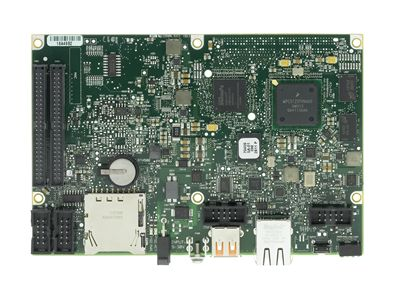
\includegraphics[width=0.7\linewidth]{sbRIO9636.jpg}
		\caption{The sbRIO 9636 board\cite{sbRIO9636Pic}}
		\label{fig:sbRIO9636}
\end{figure}


The controller consists of
\begin{itemize}
	\item 400 MHz real time processor
	\item 256 MB of system memory and 512 MB nonvolatile memory
	\item Reconfigurable Xilinx Spartan-6 LX45 FPGA
	\item 16 bit analog and digital I/O
	\item Built in USB, CAN, 10/100 Mb/s Ethernet peripherials
\end{itemize}

The board is configured through ethernet cable. The programs can be written in Labview, C or C++. We used LabView code to operate the sbRIO. The board is capable of running Real-time. %code, which is unmatched on the ROS side.

% http://sine.ni.com/nips/cds/view/p/lang/en/nid/210421

\subsection{Hardware setup}

The Endowrists, see \figref{fig:endowrits_set}, is actuated by 4 Maxon DC motors, see \secref{Maxon_Motor}. Each motor is equipped with an ESCON motor controller responsible for the cascade speed and inner loop current control. The control reference is sent through the sbRIO. They also provide current measurements to the sbRIO. Each motor hosts an encoder and a potmeter that provide absolute and relative angular position information to the FPGA built into the sbRIO board. For an graphical illustration of the connection see \figref{electro_setup}.
 
\todo{som explanation for the next line UDP, or erase it?}
The sbRIO communicates with the PC using UDP protocol. 

%\begin{figure}[H]
\begin{tikzpicture}

\node[state] (Endowrist) 
{
	%\parbox[c][2cm][c]{4cm}{\hspace{2.5em} \textbf{Endowrist}}
	\parbox[c][1.5cm][c]{2cm}{\textbf{Endowrist}}
};

\node[state,       % layout (defined above)
node distance=4cm,     
right of=Endowrist,        % Position is to the right of QUERY
yshift=+1cm] (Sensors)    % move 3cm in y
{%                     % posistion relative to the center of the 'box'
	\parbox[c][1.5cm][c]{2cm}{\textbf{Potmeters \\Encoders}}
};

\node[state,       % layout (defined above)
node distance=4cm,     
text width=4cm,        % max text width
right of=Endowrist,        % Position is to the right of QUERY
yshift=-1.5cm] (Escon)    % move 3cm in y
{%                     % posistion relative to the center of the 'box'
	\textbf{Escon controller}\\
	
	Speed control\\
	Current control\\
	Current measurement
};

\node[state,       % layout (defined above)
node distance=9.5cm,     
text width=5cm,        % max text width
right of=Endowrist,        % Position is to the right of QUERY
yshift=-0.5cm] (sbRIO)    % move 3cm in y
{%                     % posistion relative to the center of the 'box'
	\textbf{sbRIO}\\	
	 
	 .\newline\newline\newline
	
	Get control reference
	Get measurement data
	Communicate with PC\\
	
	
	
};

\node[state,       % layout (defined above)
node distance=9.5cm,     
text width=4cm,        % max text width
right of=Endowrist
] (FPGA)    % move 3cm in y
{%                     % posistion relative to the center of the 'box'
	\textbf{FPGA}\\
	
	Interface with the encoders and potmeters
	};

% draw the paths and and print some Text below/above the graph
\path (Endowrist) 	edge[bend left=20]  node[anchor=south,above]{}
node[anchor=north,below]{} (Sensors)
(Endowrist)     	edge[bend right=20] node[anchor=south,above]{} (Escon)
(Escon) edge[bend right=10] node[anchor=south,above]{} (sbRIO)
(Sensors) edge[bend left=10] node[anchor=south,above]{} (FPGA)
;


\end{tikzpicture}
\caption{Overwiev of the electronic components}
\label{electro_setup}
\end{figure} % Old picture
% \begin{figure}[H]
% \centering
% \begin{tikzpicture}
% %\draw (-1.5,-1.5) rectangle (13.5,1.5);

% \draw (-2.8,3.1) rectangle (2.8,-12.8);
% \node at (0,2.5) {\textbf{sbRIO}};


% \draw (-2.5,2) rectangle (2.5,-4.2);
% \node at (0,1.5) {\textbf{Micro processor}};
% \node[box] (datlog) at (0,0.3) {Data logging};
% \node[box] (ethcommu) at ($(0,-1.7) + (datlog)$) {Ethernet communication};
% \node[box] (shuterr) at ($(0,-1.7) + (ethcommu)$) {Shutdown:\\Communication error};


% \draw (-2.5,-4.7) rectangle (2.5,-12.6);
% \node at (0,-5.2) {\textbf{FPGA}};
% \node[box] (poscon) at ($(0,-3.3) + (shuterr)$) {Position control};
% \node[box] (enco) at ($(0,-1.7) + (poscon)$) {Encoder counter};
% \node[box] (PWM) at ($(0,-1.7) + (enco)$) {PWM control};
% \node[box] (dataES) at ($(0,-1.7) + (PWM)$) {Read data: ESCON};


% \draw (-9,-6) rectangle (-4,-12.6);
% \node[box] (spcon) at (-6.5,-8) {Speed control\\with inner current\\control};
% \node at ($(spcon) + (0,1.5)$) {\textbf{ESCON}};
% \node at ($(spcon) + (0,1.2)$) {\textbf{motor controller}};
% \node[box] (limcu) at ($(0,-1.7) + (spcon)$) {Limit output\\current};
% \node[box] (reen) at ($(0,-1.7) + (limcu)$) {Read encoder\\ticks};


% \draw (-9,-5.5) rectangle (-4,-4);
% \node at (-6.5,-4.75) {\textbf{Motor}};


% \draw (-9,-3.5) rectangle (-4,3.1);
% \node at (-6.5,2.5) {\textbf{ROS computer}};

%\node[fill = {rgb:red,1;green,2;blue,5},box] (Opt) at (0,0) {Operator};
%\node[fill = {rgb:red,1;green,2;blue,5},box] (Geo) at ($(3,0) + (Opt)$) {};
%\node[fill = {rgb:red,1;green,2;blue,5},box] (ros) at ($(3,0) + (Geo)$) {Robotic\\operating\\system};
%\node[fill = {rgb:red,1;green,2;blue,5},box] (davin) at ($(3,0) + (ros)$) {Da Vinci\\robot};
%\node[fill = {rgb:red,1;green,2;blue,5},box] (end) at ($(3,0) + (davin)$) {Endowrist};


%\draw[->, ultra thick] ([yshift=0.3cm]Opt.east) -- ([yshift=0.3cm]Geo.west);
%\draw[->, ultra thick] ([yshift=0.3cm]Geo.east) -- ([yshift=0.3cm]ros.west);
%\draw[->, ultra thick] ([yshift=0.3cm]ros.east) -- ([yshift=0.3cm]davin.west);
%\draw[->, ultra thick] ([yshift=0.3cm]davin.east) -- ([yshift=0.3cm]end.west);


%\draw[<-, ultra thick] ([yshift=-0.3cm]Opt.east) -- ([yshift=-0.3cm]Geo.west);
%\draw[<-, ultra thick] ([yshift=-0.3cm]Geo.east) -- ([yshift=-0.3cm]ros.west);
%\draw[<-, ultra thick] ([yshift=-0.3cm]ros.east) -- ([yshift=-0.3cm]davin.west);
%\draw[<-, ultra thick] ([yshift=-0.3cm]davin.east) -- ([yshift=-0.3cm]end.west);

%\node at (1.5,1) {Position};
% \node at (4.5,1) {Position};
% \node at (7.5,1) {yes};
% \node at (10.5,1) {yes};

%\node at (1.5,-1) {Force};
% \node at (4.5,1) {Position};
% \node at (7.5,1) {yes};
% \node at (10.5,1) {yes};
%\end{tikzpicture}
%\caption{Overall system with feedback in both direction}
%\end{figure}



\begin{figure}[H]
\centering
\tikzset{dataset/.style = {rectangle, draw, text width = 5.5cm, minimum height=3cm}}
\begin{tikzpicture}

\node [dataset] (mpro) at (0,3) {\textbf{Micro processor}
\begin{itemize}[itemsep=0pt,partopsep=0pt,topsep=0pt]
\item Data logging
\item Ethernet communication
\item Shutdown: Communication error \\
\end{itemize}};

\node [dataset, below of=mpro, node distance=6.5cm] (FPGA) {\textbf{FPGA}
\begin{itemize}[itemsep=0pt,partopsep=0pt,topsep=0pt] 
\item Position contron
\item Encoder counter
\item PWM control
\item Read data: Escon 
\end{itemize}};

\draw[->, ultra thick] ([xshift=-1cm]mpro.south) -- ([xshift=-1cm]FPGA.north);
\draw[<-, ultra thick] ([xshift=1cm]mpro.south) -- ([xshift=1cm]FPGA.north);

\node [dataset, left of=FPGA, node distance=7cm] (emc) {\textbf{ESCON motor controller}
\begin{itemize}[itemsep=0pt,partopsep=0pt,topsep=0pt] 
\item Speed controll with intter current control
\item Limit output current
\item Read encoder ticks 
\end{itemize}};

\draw[->, ultra thick] ([yshift=-1cm]emc.east) -- ([yshift=-1cm]FPGA.west);
\draw[<-, ultra thick] ([yshift=1cm]emc.east) -- ([yshift=1cm]FPGA.west);

\tikzset{dataset/.style = {rectangle, draw, text width = 6cm, minimum height=10.5cm}}
\node [dataset, above of=FPGA, node distance=3.5cm] (motor) {\textbf{sbRIO}
\begin{itemize}[itemsep=0pt,partopsep=0pt,topsep=260pt] % Edit the last number to fit title 
\item[]  %  This line is necessary!!
\end{itemize}};


\tikzset{dataset/.style = {rectangle, draw, text width = 5.5cm, minimum height=1cm}}
\node [dataset, above of=emc, node distance=2.5cm] (motor) {\textbf{Motor}};

\draw[->, ultra thick] ([xshift=-1cm]motor.south) -- ([xshift=-1cm]emc.north);
\draw[<-, ultra thick] ([xshift=1cm]motor.south) -- ([xshift=1cm]emc.north);

\tikzset{dataset/.style = {rectangle, draw, text width = 5.5cm, minimum height=5cm}} % This edits the size of the Ros computer box 
\node [dataset, above of=motor, node distance=3.75cm] (ROS) {\textbf{Ros computer}
\begin{itemize}[itemsep=0pt,partopsep=0pt,topsep=0pt] 
\item 1
\item 2
\item 3 
\end{itemize}};

\draw[->, ultra thick] ([yshift=-1cm]mpro.west) -- ([yshift=-1cm]ROS.east); % ([yshift=-1cm]ROS.west) should probaly be edited!!!
\draw[<-, ultra thick] ([yshift=1cm]mpro.west) -- ([yshift=1cm]ROS.east);

% \draw [->,ultra thick] (-1,1.5) -- (-1,-2); %Micro to FPGA
% \draw [<-,ultra thick] (1,1.5) -- (1,-2);

% \draw [->,ultra thick] (-3,-3) -- (-4,-3);
% \draw [<-,ultra thick] (-3,-4) -- (-4,-4);

\end{tikzpicture}
\caption{Say somthing cool- "\textit{Somthing cool!}"}
\end{figure}

\todo{Include arrow, label anc new caption... elaborate this picture breifly, what do the different boxes do?}

% \begin{figure}[htb]
% \tikzset{dataset/.style = {rectangle, draw, text width = 5cm, minimum height=1in}}
% \begin{tikzpicture}[auto, font={\scriptsize}]
%     % Place nodes
%     \node [dataset] (tm) {Data 1 
%                             \begin{itemize}[itemsep=0pt,partopsep=0pt,topsep=0pt]   %% this added.
%                                 \item{\# Adults } 
%                                 \item{\# Children} 
%                                 \item{Income}
%                                 \item{Ethnicity}
%                             \end{itemize}\par};
%     \node [dataset, right of=tm, node distance=3in] (dmv) {Data 2 
%                             \begin{itemize}[itemsep=0pt,partopsep=0pt,topsep=0pt] 
%                                 \item{Data 2} 
%                             \end{itemize}\par};
%     % draw links
%     \path [<->] (tm) edge node[above, sloped] {Address} (dmv);
% \end{tikzpicture}
%     \caption{Analysis dataset assembly.}
%     \label{fig:dataset}
% \end{figure}


\subsection{Motor}\label{Maxon_Motor}
The four motors for actuating the Endowrist is sold as a bulk solution which include motor, gear and a position encoder, see \figref{fig:Full_motor _dis}.

The control of these motors are done through the ESCON motor drivers, which are connected to the sbRIO board. The datasheet for the motor parts can be found on \path{CD:/Datasheets/Motor/}\todo{(Datasheet) Don't know if this is necessary - Maby we don't have to turne in a physical paper??}

%The ESCON motor controllers are attached to the sbRIO controller and send the control signals through cables. The motor has a nominal torque of 6.96 mNm.
%4 Maxon motors are used for the actuation of the endowrist. The motors are implemented using a combination gear (Maxon 353816) including the gearing, the servo motor and the sensors. The ESCON motor controllers are attached to the sbRIO controller and send the control signals through cables. The motor has a nominal torque of 6.96 mNm.

\begin{figure}[H]
	\centering
	\begin{subfigure}{.32\textwidth}
		\vspace{0pt}
		\centering
		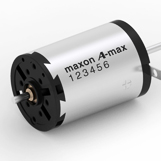
\includegraphics[width=\linewidth]{motor.jpg}
		\caption{The Maxon 110160 \newline DC motor\cite{motor_motor}}
		\label{fig:motor}
	\end{subfigure}
	\begin{subfigure}{.32\textwidth}
		\centering
		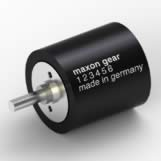
\includegraphics[width=\linewidth]{motor_gear.jpg}
		\caption{The planetary gearhead equipped with sleeve bearing\cite{motor_gear}}
		\label{fig:motor_gear}
	\end{subfigure}
	\begin{subfigure}{.32\textwidth}
	\hspace{5pt}
		\centering
		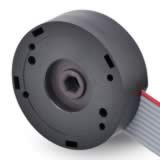
\includegraphics[width=\linewidth]{motor_sensor.jpg}
		\caption{The encoder used for getting angular data\cite{motor_encoder}}
		\label{fig:motor_sensor}
	\end{subfigure}
	\caption{The combination gear disassembled}
	\label{fig:Full_motor _dis}
\end{figure}






\subsection{ESCON 50/5 motor controller}
For driving the motors, there has been implemented four ESCON motor driver of the type 50/5 (part number 438725), see \figref{fig:ESCON505}. 

\begin{figure}[H]
	\centering
		\centering
		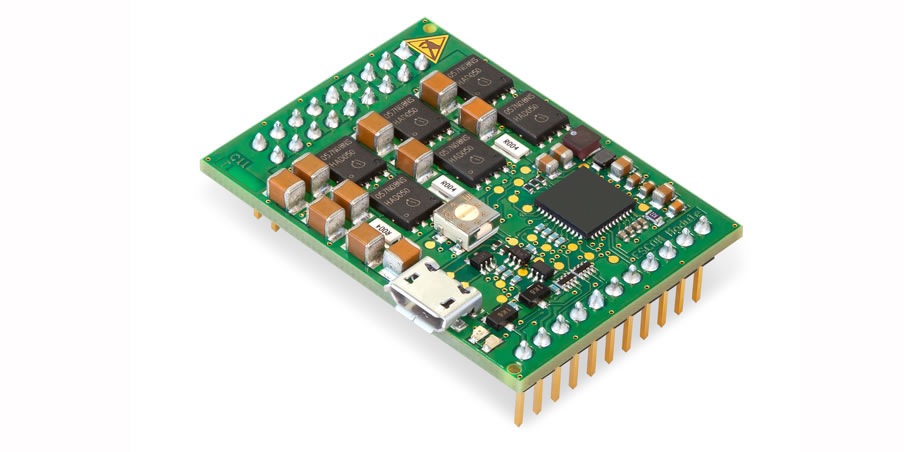
\includegraphics[width=0.7\linewidth]{ESCON505.jpg}
		\caption{ESCON 50/5 DC motor controller\cite{ESCON_motor_controller}}
		\label{fig:ESCON505}
\end{figure}

These are controllers for permanent magnet-activated bushed DC motors an can deliver a power up to 250 Watt for the motor connected to the controller. 

It has three operating modes

\begin{itemize}
\item Current controller
\item Speed controller (open loop)
\item Speed controller (closed loop)
\end{itemize}

\todo{We need to decide what type of controller we are going with and why?}



\section{Mechanical test setup}\label{sec:Mechanical_testsetup.tex}
The mechanical test setup available at Aalborg University can be seen on \figref{fig:Mec_abcd}. It includes four of the motors described in \secref{Maxon_Motor} attached to the four rotational plates seen on \figref{fig:Mec_a} and \figref{fig:Mec_b}. These plates connect the motors and the Endowrist, such that the EndoWrist can be manipulated. See \figref{fig:Mec_c} and \figref{fig:Mec_d} for the attachment of the Endowrist to the EndoWrist holder.  

\begin{figure}[H]
	\centering
	\begin{minipage}[t]{0.9\textwidth}
	\begin{subfigure}{0.45\textwidth}
		\vspace{-10pt}
		\centering
		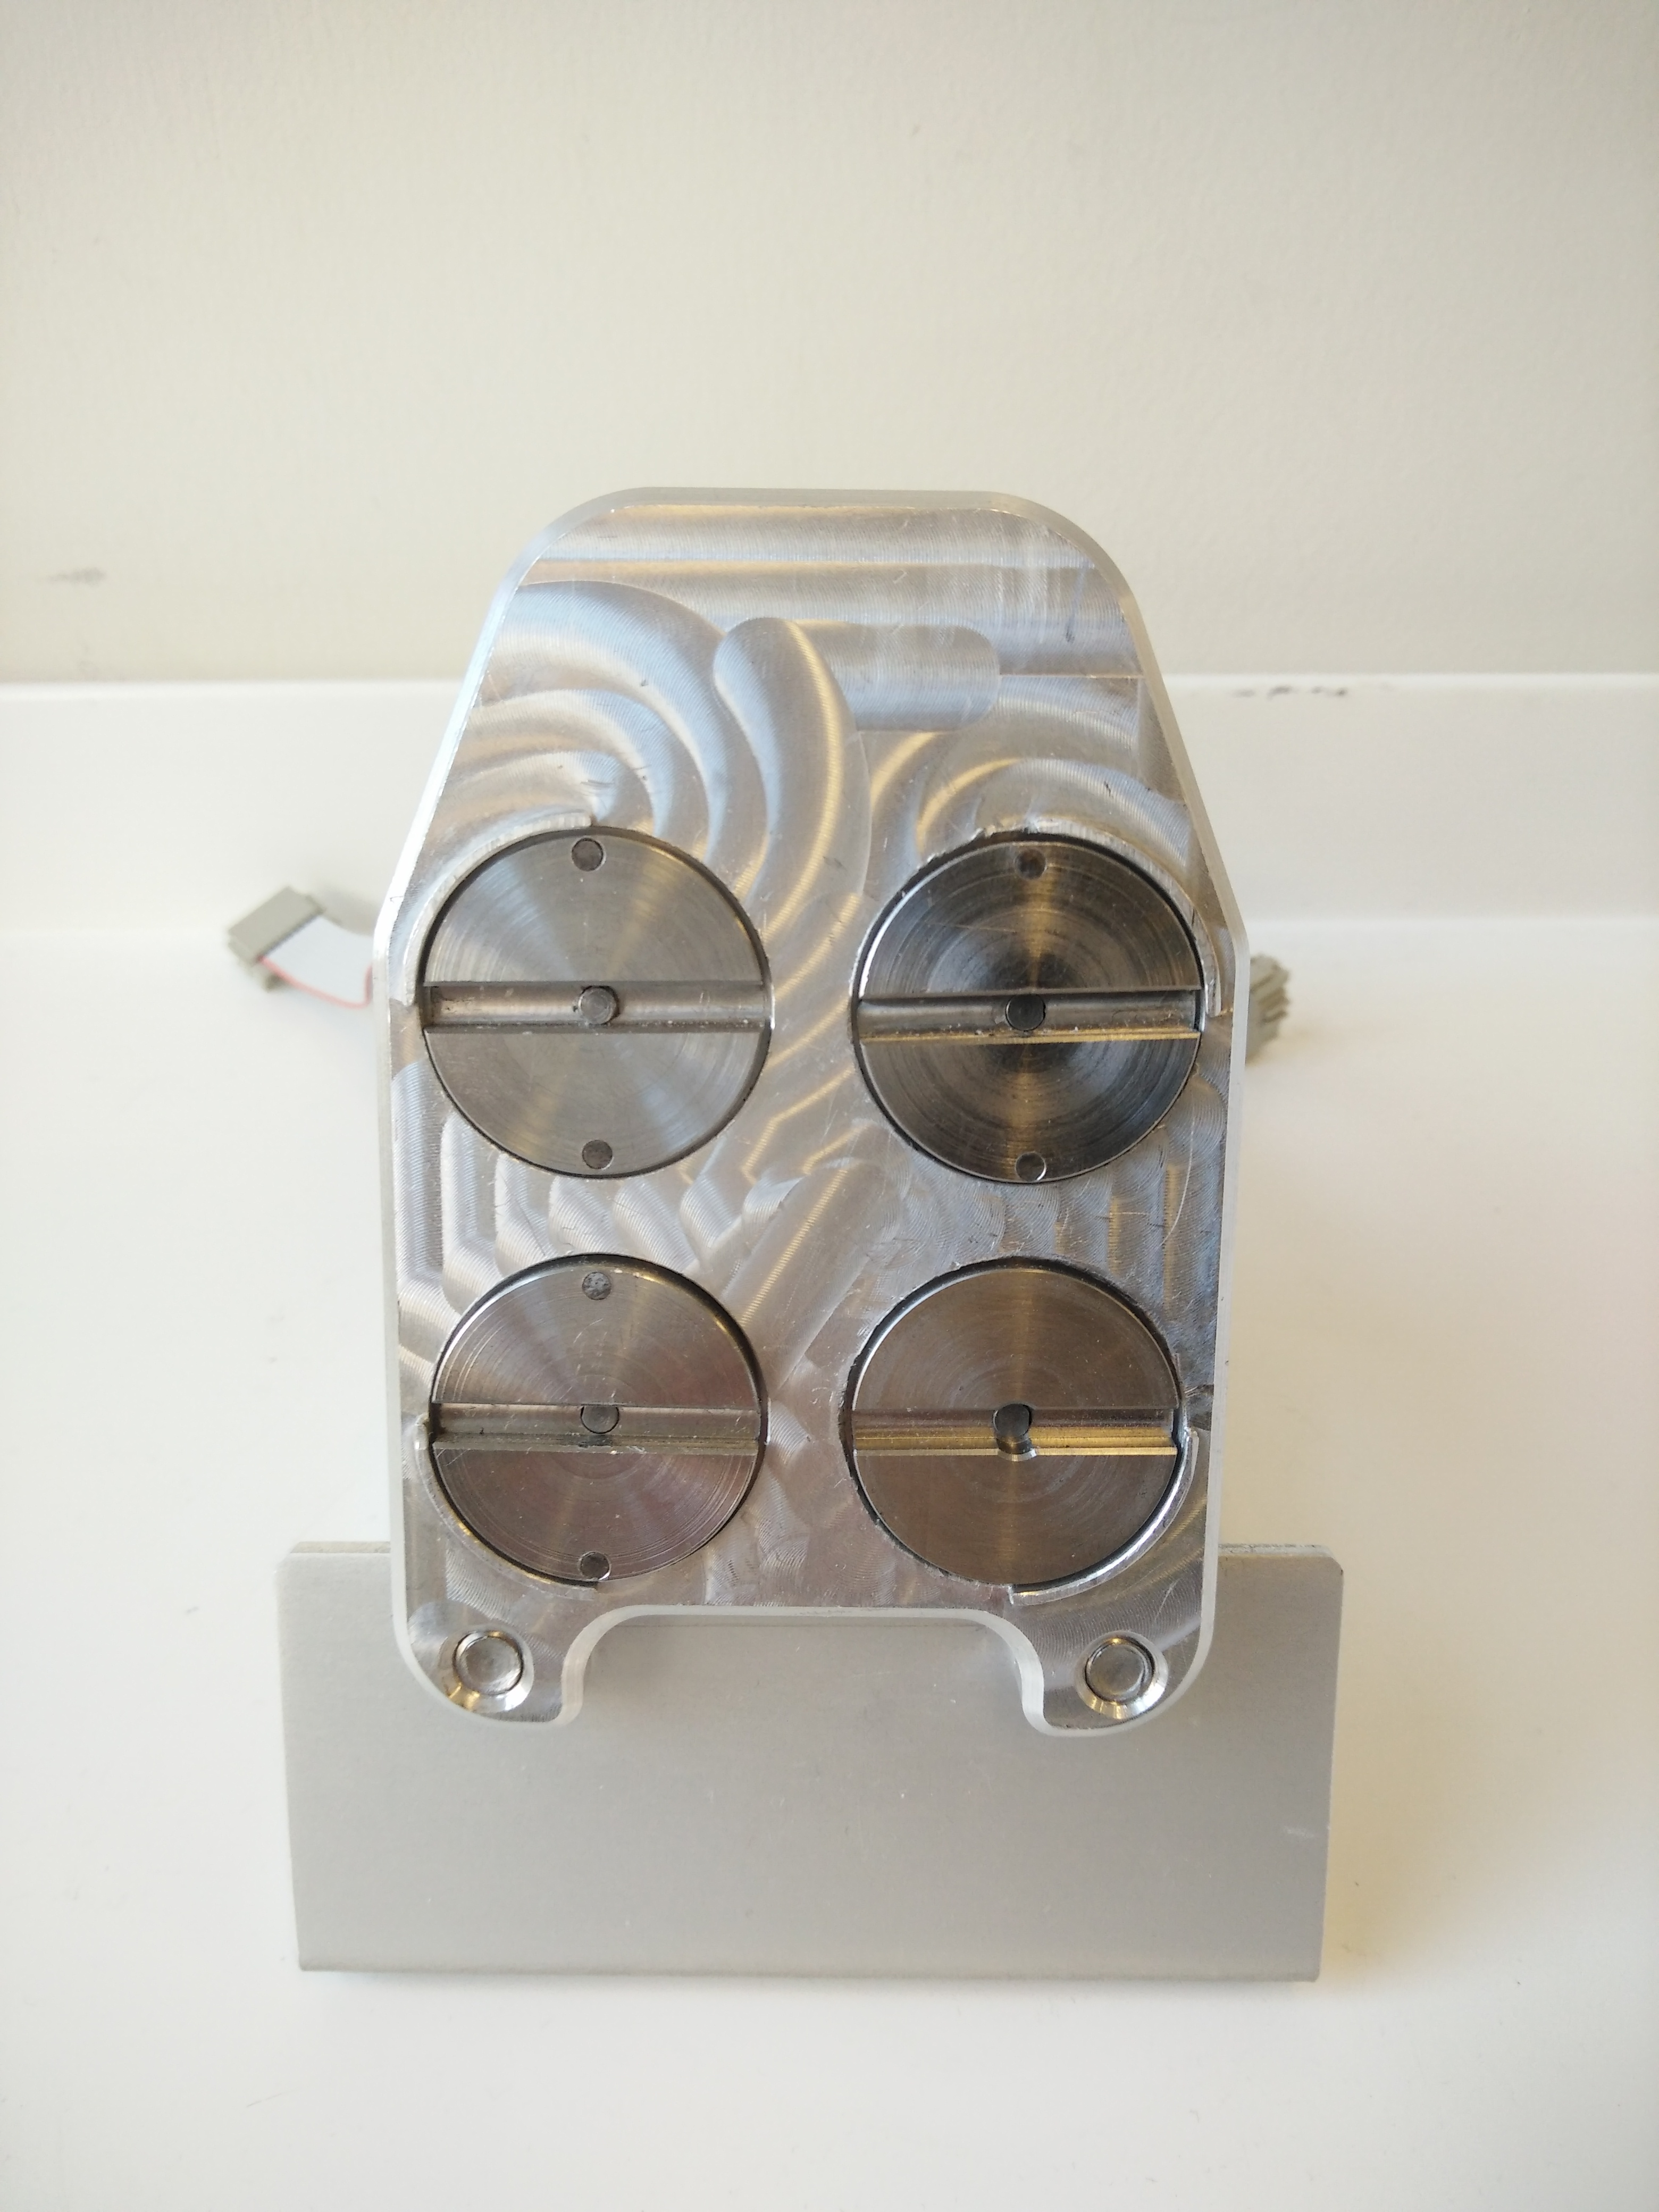
\includegraphics[width=\linewidth]{Test_setup1.jpg}
		\caption{EndoWrist holder. Front view}
		\label{fig:Mec_a}
	\end{subfigure}
	\hspace{\fill}
	\begin{subfigure}{0.45\textwidth}
		\centering
		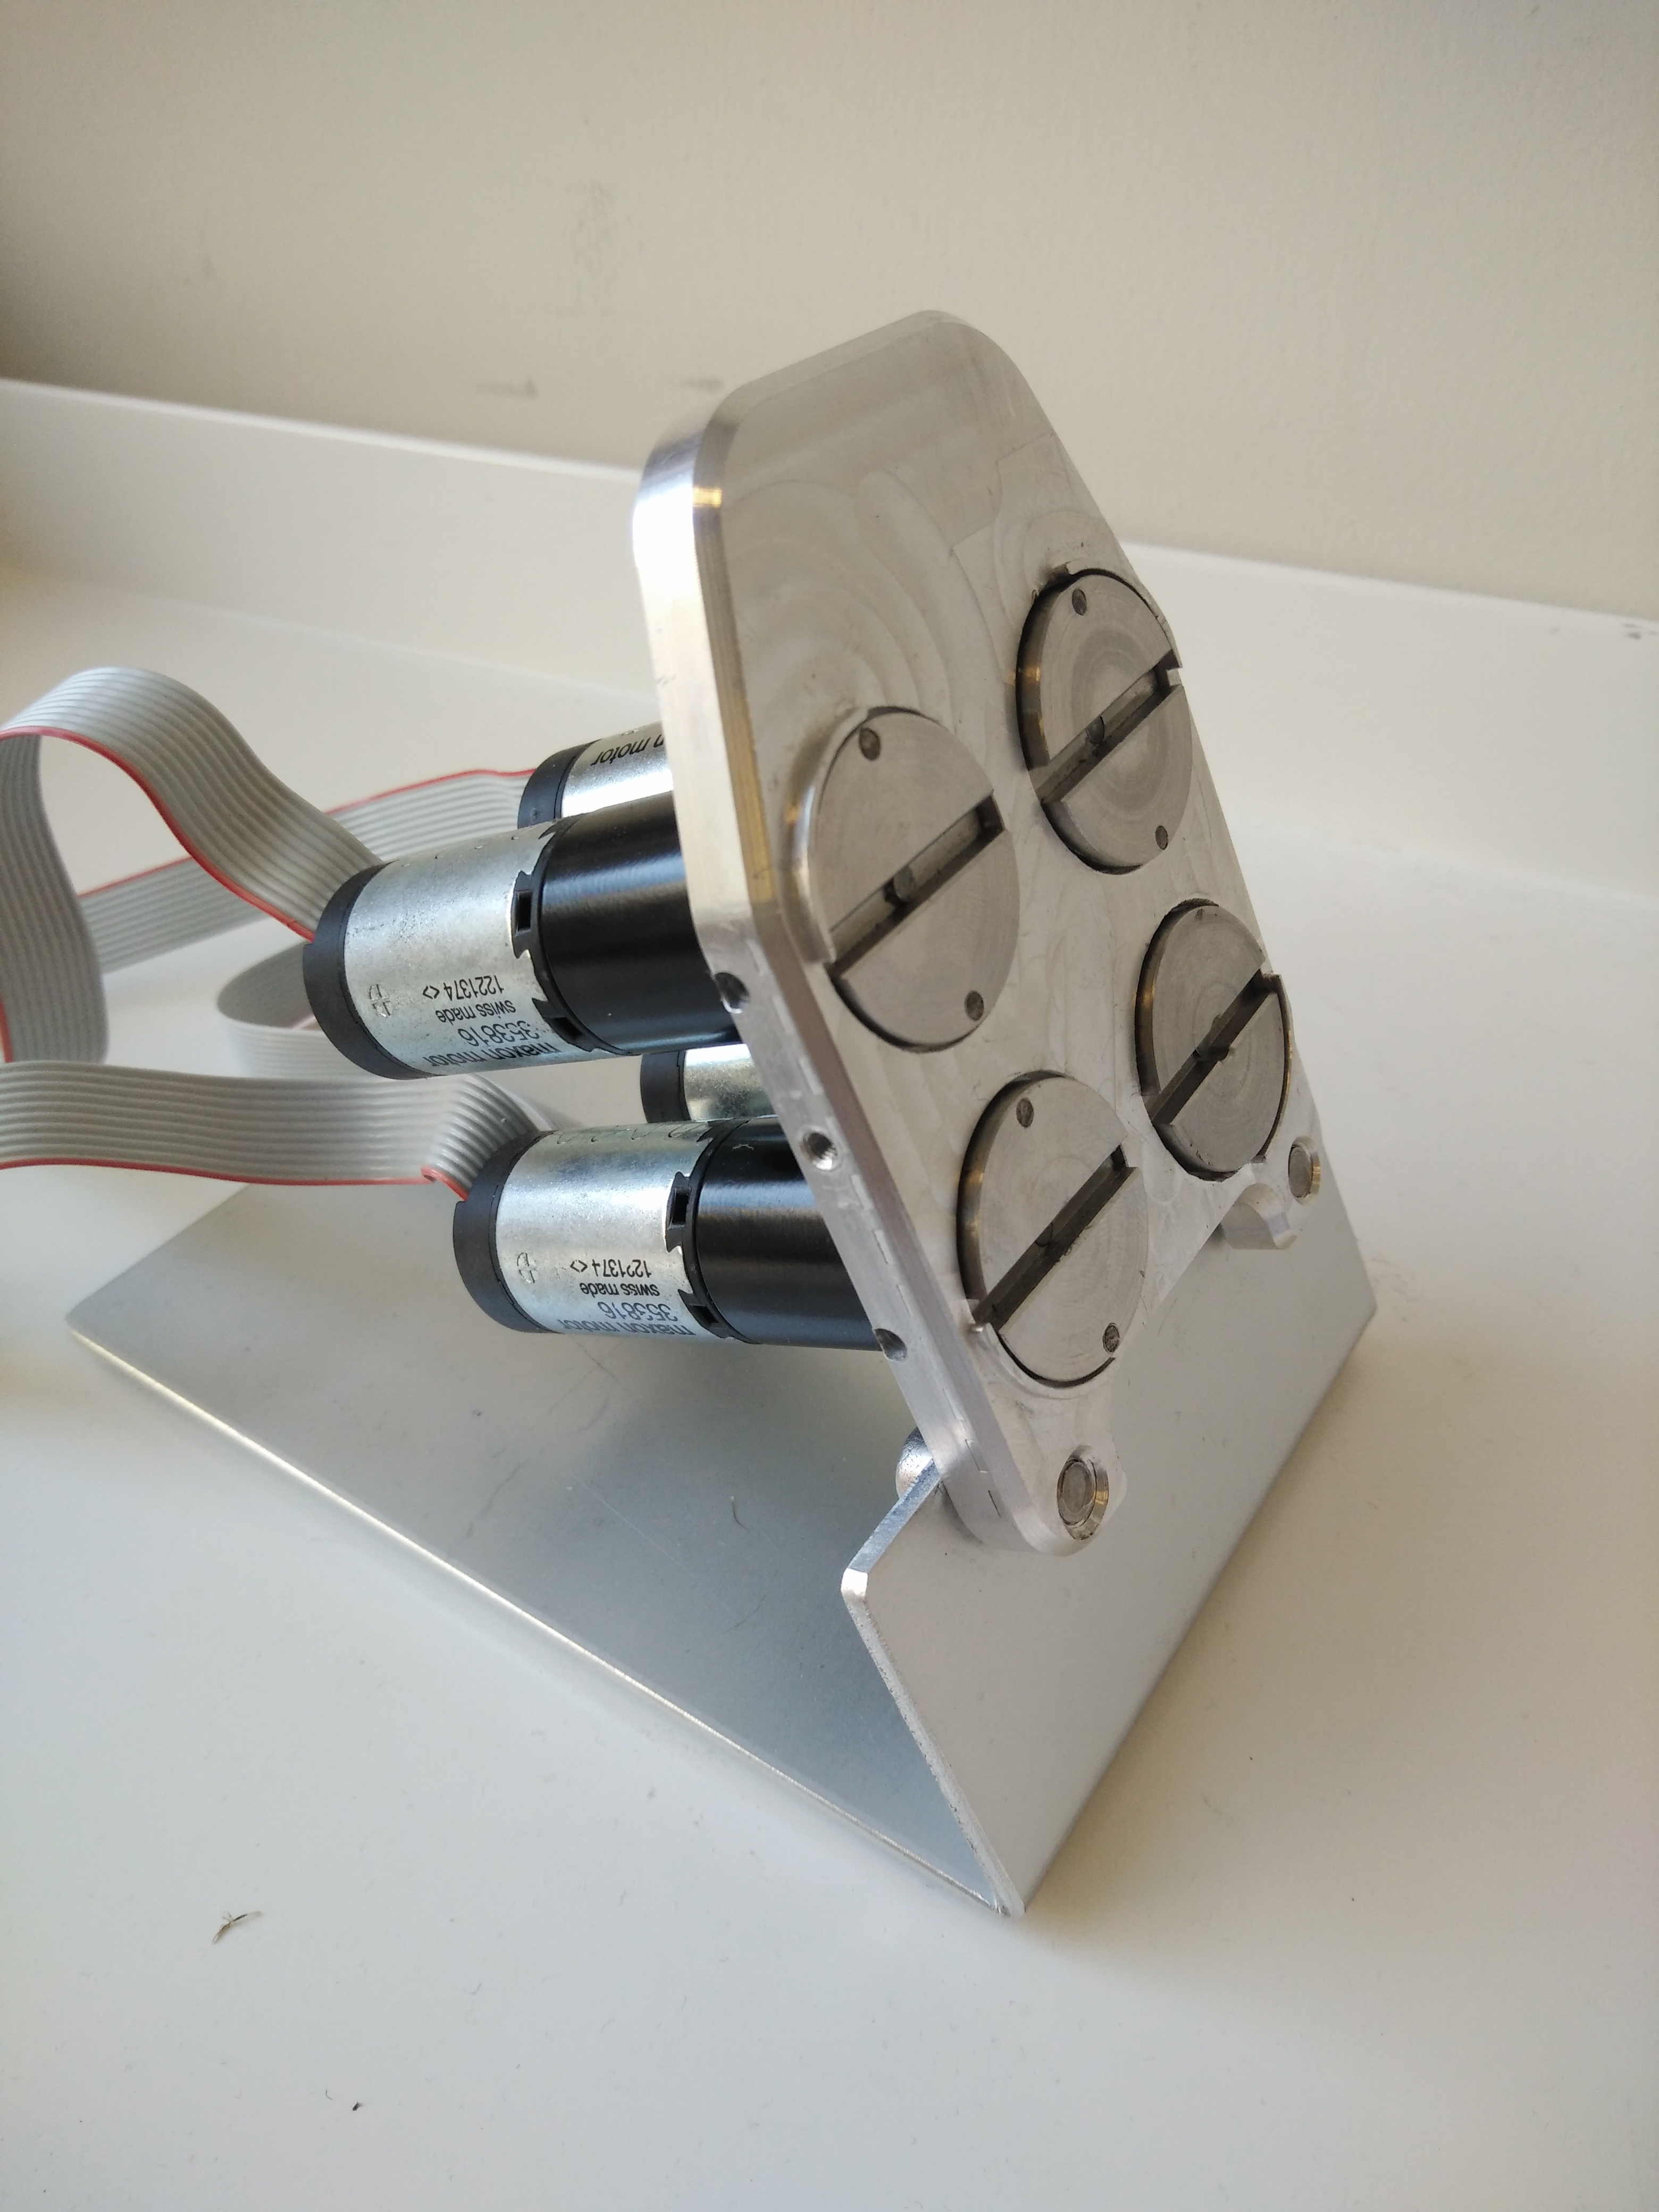
\includegraphics[width=\linewidth]{Test_setup2.jpg}
		\caption{EndoWrist holder with motors at the back. Side view}
		\label{fig:Mec_b}
	\end{subfigure}
	\end{minipage}

	\begin{minipage}[t]{0.9\textwidth}
	\vspace{20pt}
	\begin{subfigure}{0.45\textwidth}
		\vspace{0pt}
		\centering
		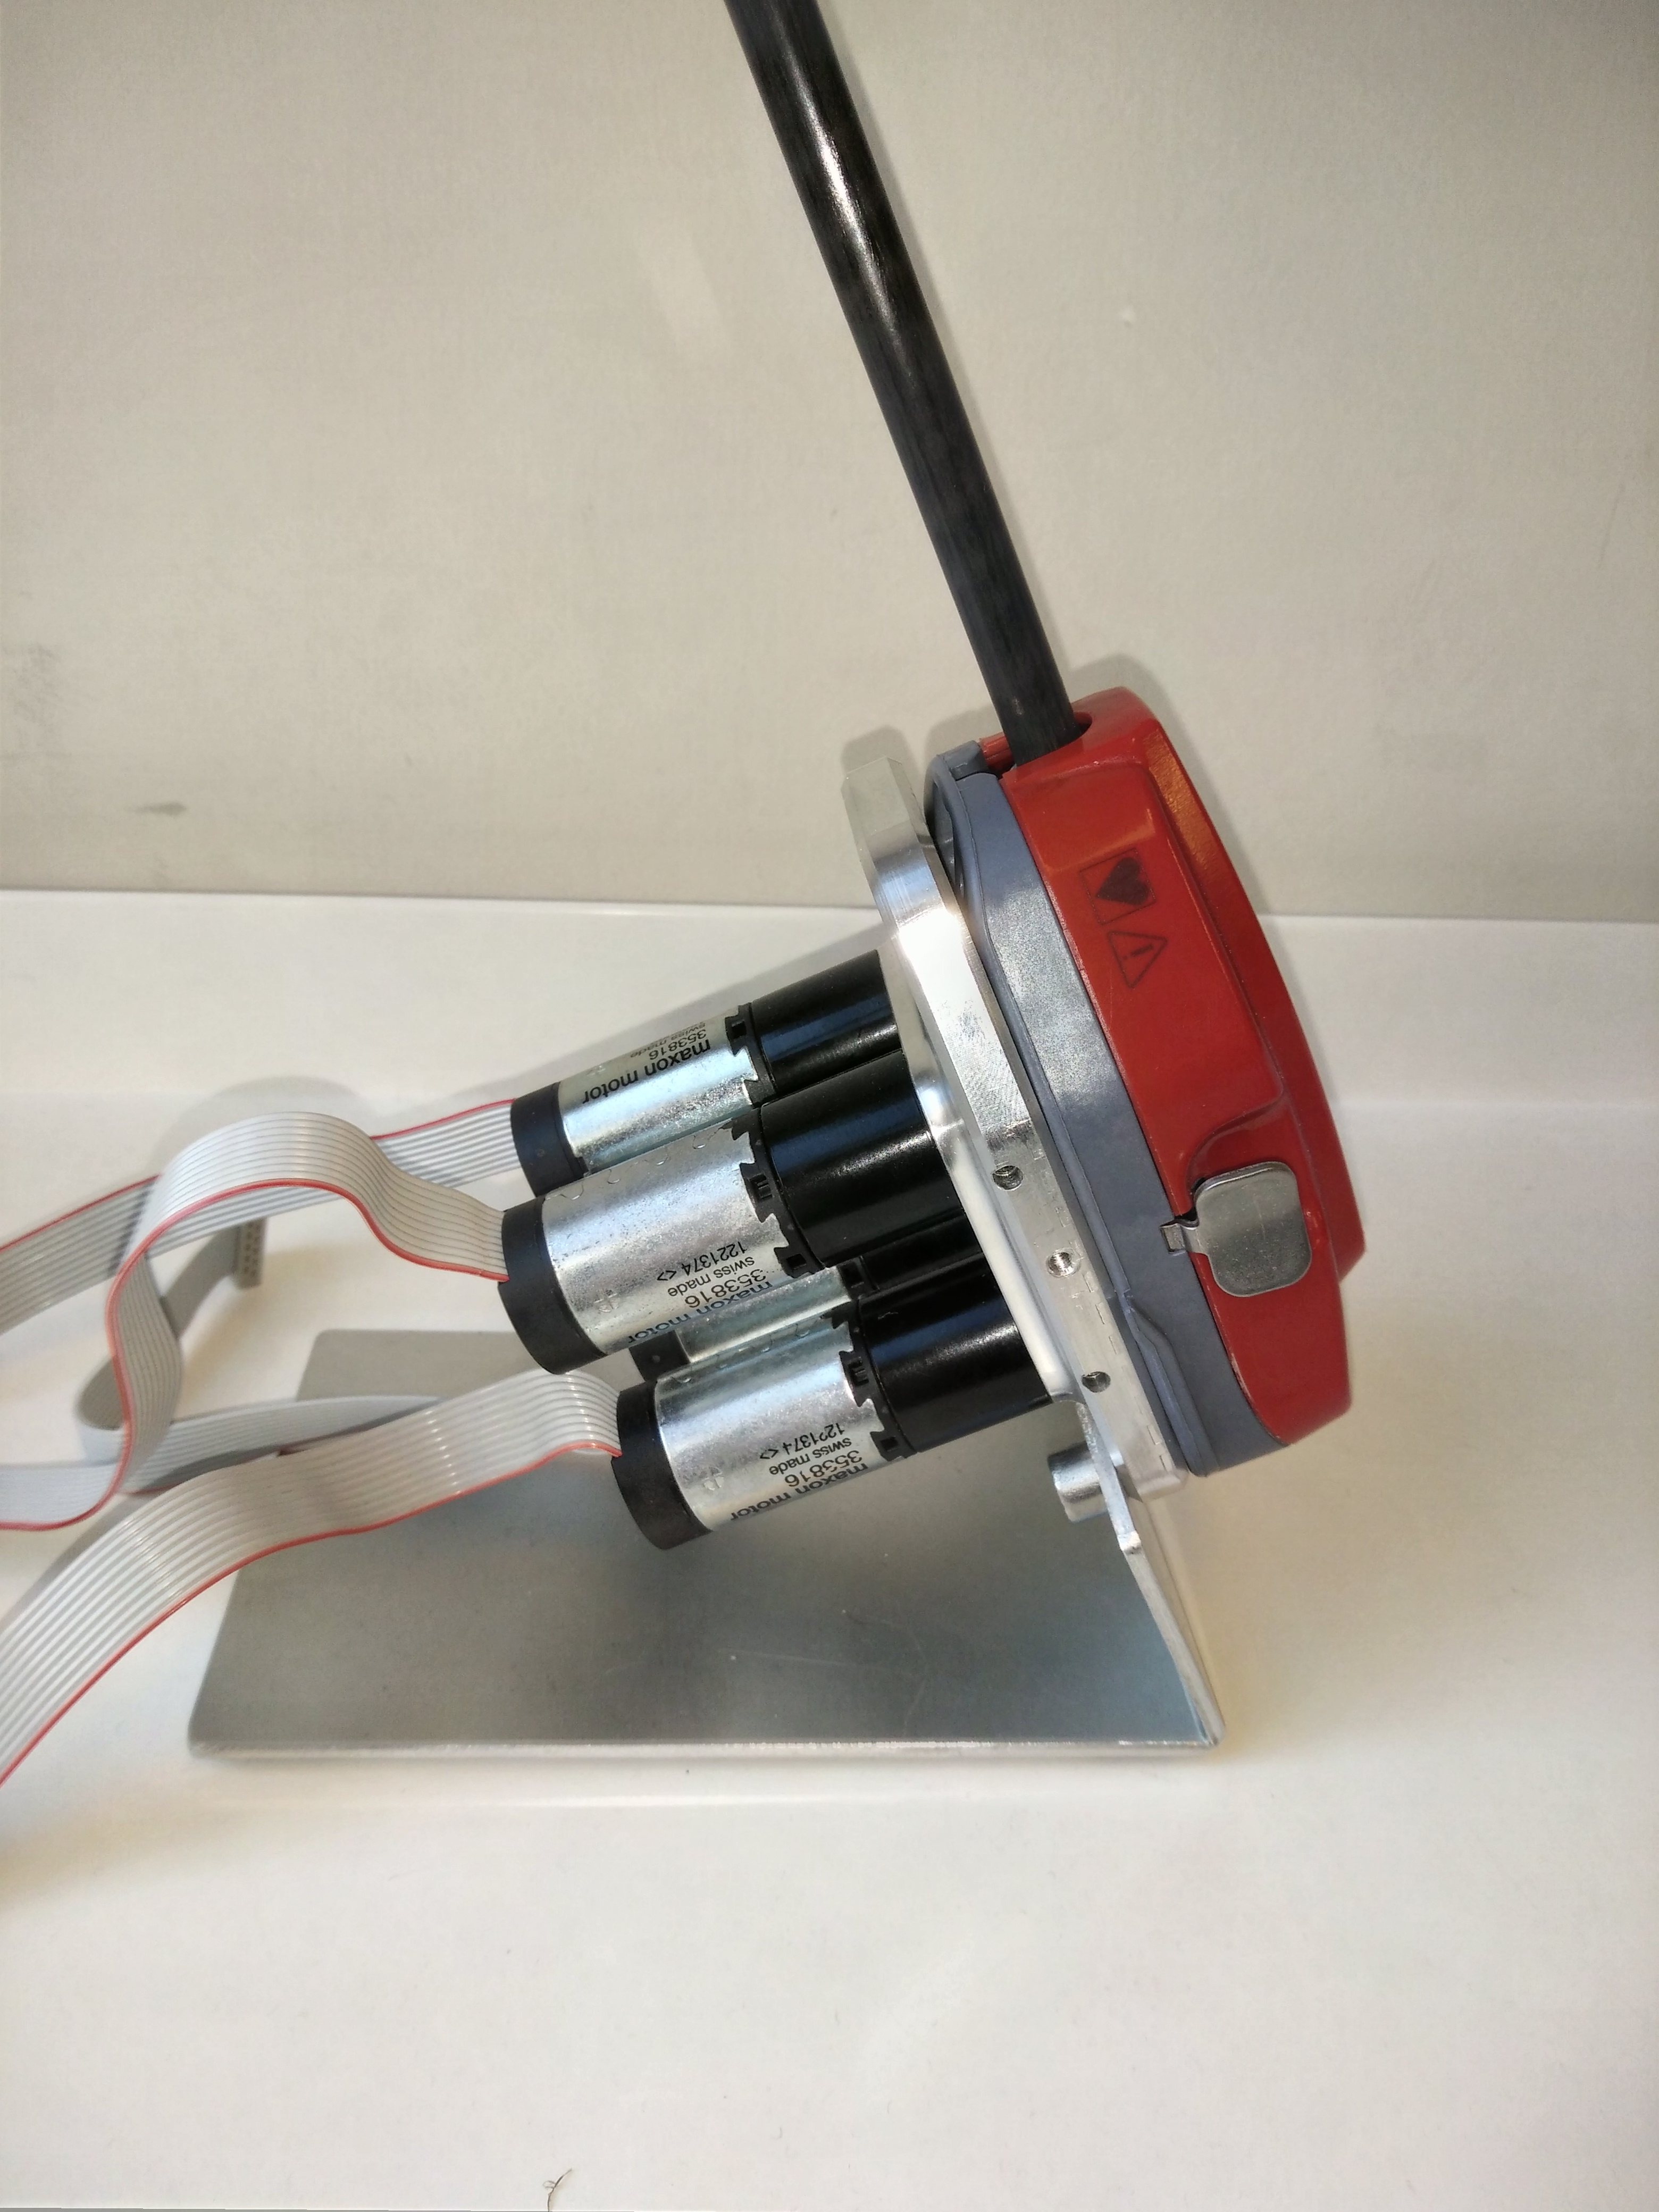
\includegraphics[width=\linewidth]{Test_setup3.jpg}
		\caption{EndoWrist holder with EndoWrist and motors. Side view}
		\label{fig:Mec_c}
	\end{subfigure}
	\hspace{\fill}
	\begin{subfigure}{0.45\textwidth}
		\centering
		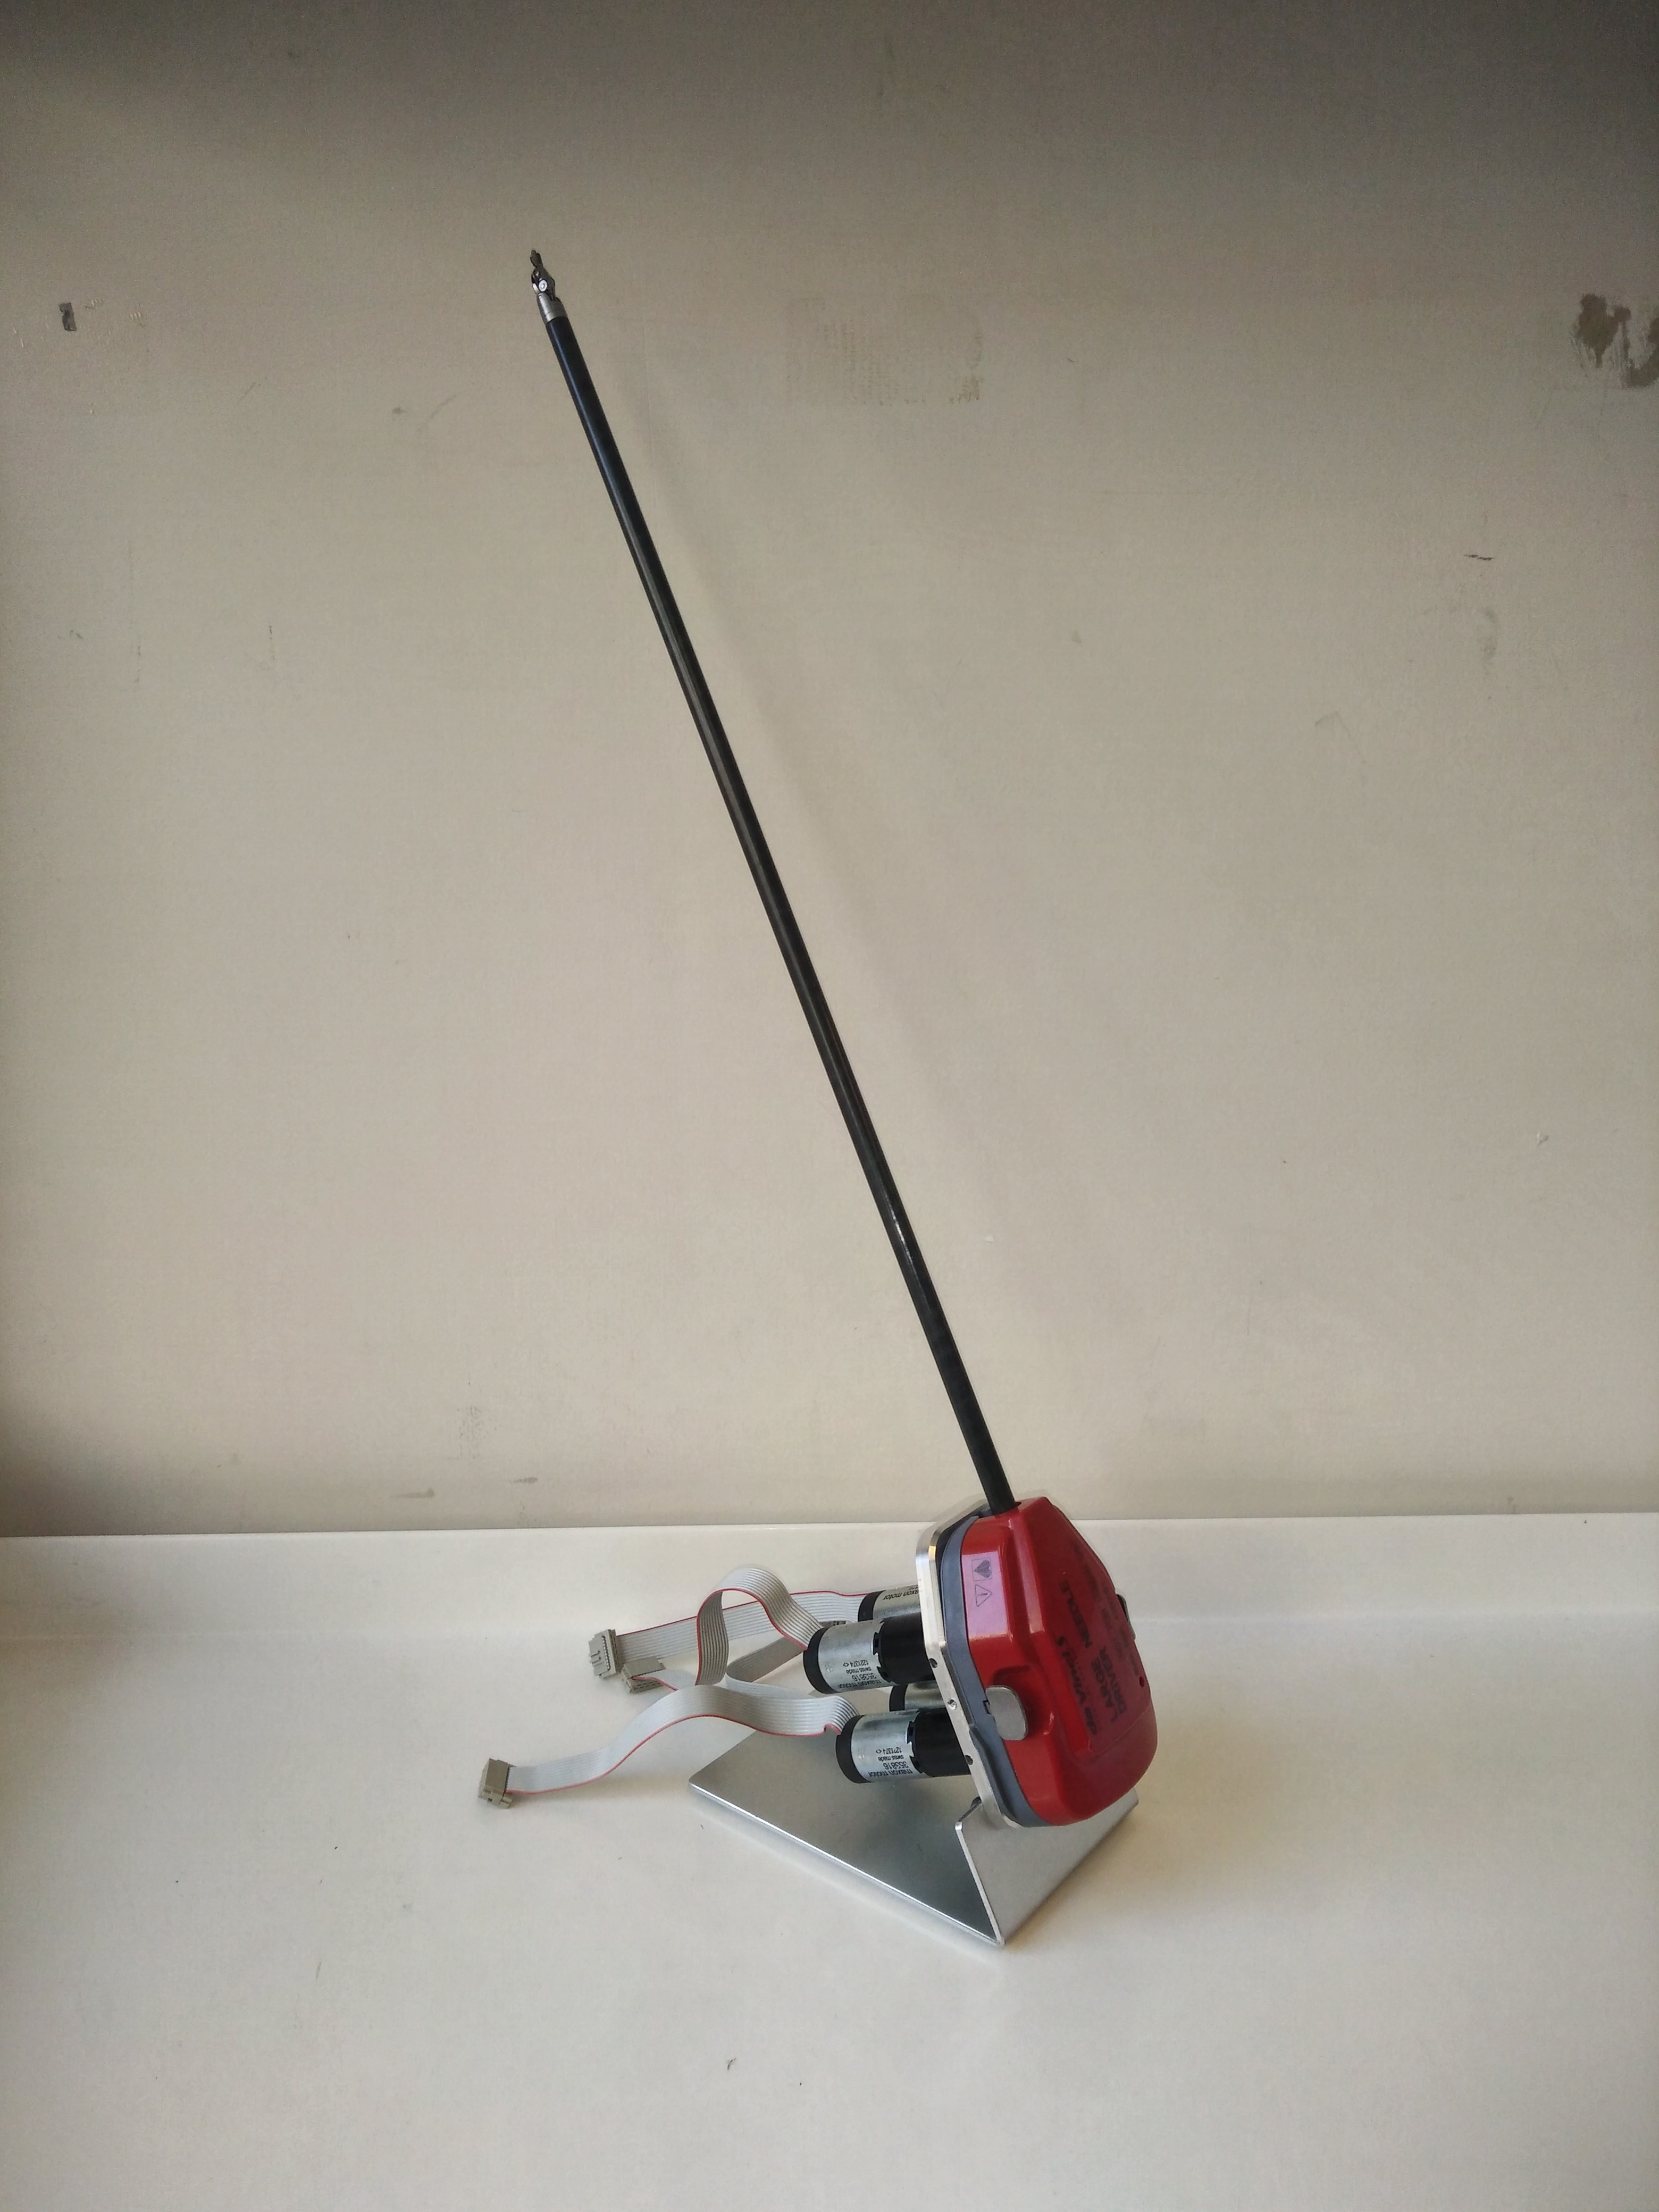
\includegraphics[width=\linewidth]{Test_setup4.jpg}
		\caption{Full view of the mechanical test setup}
		\label{fig:Mec_d}
	\end{subfigure}
	\end{minipage}

	\caption{Four pictures of the mechanical test setup available at Aalborg University, which include motors, EndoWrist and EndoWrist holder}
	\label{fig:Mec_abcd}
\end{figure}

This setup can manipulate the EndoWrist in the same manner as if the tool was connected to the da Vinci robot, see \secref{sec:da_vin_rob}.
\todo{Does this last line explaine what the setup can do in a proper manner?}


\section{Geomagic touch}\label{sec:geo_magic}
The Geomagic Touch(GT) is a haptic feedback controller device, %\textcolor{red}{which has the ability to manipulate its joints in such a way that the user feels resistance when moving the pin in a certain direction or way.}
\textcolor{green}{that is able to output force to the user, and arbitrarily resist the user's attempts at moving the controller.
	} The Geomagic Touch described in this section can be seen on \figref{fig:phantom_omni}.

\begin{figure}[H]
	\centering
	\begin{subfigure}{.45\textwidth}
		\centering
		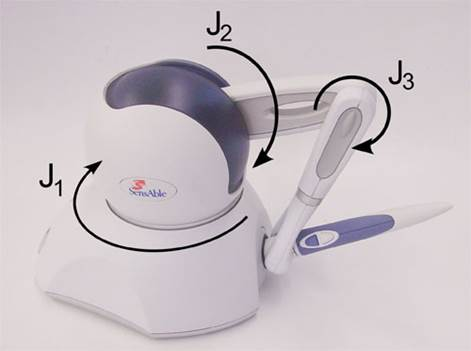
\includegraphics[width=\linewidth]{haptick1.png}
		\caption{Overview of the Geomagic Touch's first three joints.}
		\label{fig:phantom1}
	\end{subfigure}
	\begin{subfigure}{.45\textwidth}
		\centering
		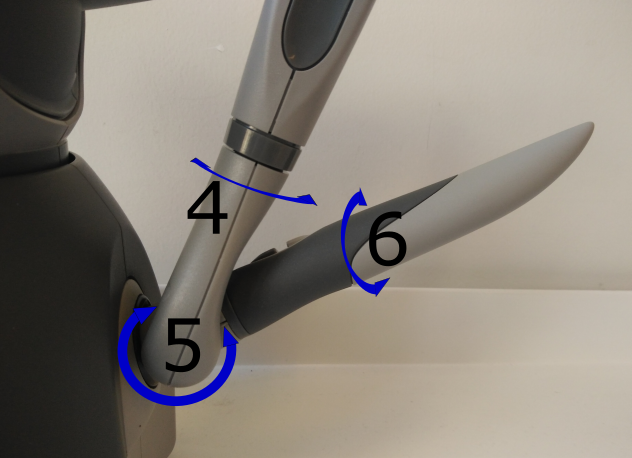
\includegraphics[width=\linewidth,height=5.4cm]{haptick2.png}
		\caption{Overview of the Geomagic Touch's last three joints}
		\label{fig:phantom2}
	\end{subfigure}
\caption{Overview of all the Geomagic Touch's joints.}
\label{fig:phantom_omni}
\end{figure}

 On \figref{fig:phantom_omni}, it can be seen that the Geomagic Touch has six \gls{DOF}, where only the first three can be actuated, see \figref{fig:phantom1}. This means that the device only has the ability to generate translational force feedback with three \gls{DOF}.% in this case roll, pitch and yaw.

The GT communicates with the computer through User Datagram Protocol (UDP). This communication can be established directly through an ethernet cable or by plugging the ethernet cable into USB converter. The interfacing is shown on \figref{interface}. The Geomagic Touch was programmed and the connection was established using a C++ based application programming interface (API). The API provides force rendering,  virtual environment and position measurement features. The present project utilizes force rendering capabilities to provide force feedback and measures the GT's position as an input to the system.

\section{Overview}
As mentioned before, a fully featured DaVinci robot has four arms with 6-7 \gls{DOF} in total, when the Endowrist instrument included.
%Since the robot has 4 arms, there are 4 instruments.
%Although our setup controls only 4 motors, in funcionality it is equivalent to one DaVinci arm.
Although our setup controls only 4 motors, it can manipulate the surgical tool itself in the same way the da Vinci robot does. The missing features are the one related to the hand of the robot holding the tool.

The sbRio board controls the test setup and as such represents the onboard computer on the DaVinci robot.
In order to perform higher level functions such as force feedback control, it is necessary to remotely handle data and send high-level commands.
This is handled by an external computer system that is connected to the Geo magic touch device.

The sbRIO board and the Geomagic Touch both communicate with the computer using UDP.
The computer also performs force estimation using a dynamical model of the test setup (or EndoWrist, more precisely), this is vital for force feedback.
In order to connect software components responsible for communicating with hardware and the ones responsible for the control algorithm and estimation.
For this purpose we use the Robot Operating System (ROS), which uses a network architecture to share data between components via data streams.

\begin{figure}[H]
\begin{tikzpicture}
\draw (-1.5,-2.5) rectangle (13.5,2.5);


\node[box] (Opt) at (0,0) {Operator};
\node[box] (Geo) at ($(3,0) + (Opt)$) {Geomagic\\touch};
\node[box] (ros) at ($(3,0) + (Geo)$) {Robotic\\operating\\system};
\node[box] (davin) at ($(3,0) + (ros)$) {Embedded \\system};
\node[box] (end) at ($(3,0) + (davin)$) {Endowrist};


\draw[->, ultra thick] ([yshift=0.3cm]Opt.east) -- ([yshift=0.3cm]Geo.west);
\draw[->, ultra thick] ([yshift=0.3cm]Geo.east) -- ([yshift=0.3cm]ros.west);
\draw[->, ultra thick] ([yshift=0.3cm]ros.east) -- ([yshift=0.3cm]davin.west);
\draw[->, ultra thick] ([yshift=0.3cm]davin.east) -- ([yshift=0.3cm]end.west);


\draw[<-, ultra thick] ([yshift=-0.3cm]Opt.east) -- ([yshift=-0.3cm]Geo.west);
\draw[<-, ultra thick] ([yshift=-0.3cm]Geo.east) -- ([yshift=-0.3cm]ros.west);
\draw[<-, ultra thick] ([yshift=-0.3cm]ros.east) -- ([yshift=-0.3cm]davin.west);
%\draw[<-, ultra thick] ([yshift=-0.3cm]davin.east) -- ([yshift=-0.3cm]end.west);

\node at (1.5,1) {Position};
\node at (4.5,1) {Position};
% \node at (7.5,1) {yes};
% \node at (10.5,1) {yes};

\node at (1.5,-1) {Force};
\node at (4.5,-1) {Force};
\node at (10.5,1) {Torque};
% \node at (10.5,1) {yes};
\node at (7.5,1.5) {Motor enable};
\node at (7.5,1) {Position};
\node at (7.5,-1) {Position};
\node at (7.5,-1.5) {Speed};
\node at (7.5,-2) {Current};

\end{tikzpicture}
\caption{Overall system with feedback in both direction}
\end{figure}
\todo{Do we have a model of the operator?}

\subsection*{Problem formulation}
\begin{itemize}
\item \textit{How can the communication speed be increased to at least 600 Hz, such that force feedback can be implement on the system?}
\item \textit{How is a controller to be designed such that it can handle delay in the system?}
\end{itemize}
\todo{Problemformulation}